%==============================================================================
% OrgMemBench --- Datasets-and-Benchmarks paper
%==============================================================================
%
% WORKING TITLE (placeholder, confirm before submission):
%   "OrgMemBench: A Benchmark for Long-Horizon Organizational Memory in AI Agents"
%
% This is the ASSEMBLED paper. The body is composed of \input{sections/<name>}
% fragments; the preamble, title/author block, and tooling are inherited from
% the original scaffold (structure follows docs/publishing-a-paper-2026.md
% section 5.3; tooling follows section 5.1).
%
%------------------------------------------------------------------------------
% DOCUMENT CLASS --- PLACEHOLDER
%------------------------------------------------------------------------------
% This uses the always-available `article` class so the paper compiles with any
% TeX install (tectonic / pdflatex / latexmk) and needs no venue style download.
%
% >>> SWAP to neurips_2026.sty / iclr2026.sty when targeting a venue <<<
%     see docs/publishing-a-paper-2026.md section 1.1 for the template URLs.
%     NeurIPS 2026 -> neurips_2026.sty (\usepackage{neurips_2026})
%     ICLR  2026   -> iclr2026.sty     (\usepackage{iclr2026_conference})
% When you swap, delete the geometry line below (venue .sty sets margins),
% and move the title/author block into the venue macros.
%------------------------------------------------------------------------------
\documentclass[11pt]{article}

\usepackage[letterpaper,margin=1in]{geometry}
\usepackage[T1]{fontenc}
\usepackage[utf8]{inputenc}
\usepackage{microtype}

\usepackage{amsmath}
\usepackage{amssymb}
\usepackage{graphicx}      % include figures (with alt-text for arXiv HTML, see guide 1.1)
\usepackage{booktabs}      % professional tables, no vertical rules (guide 1.6)
\usepackage{siunitx}       % decimal-aligned numbers in tables (guide 1.6 / 5.1)
\usepackage{xcolor}
\usepackage{caption}
\usepackage{subcaption}
\usepackage[numbers,sort&compress]{natbib}   % BibTeX; matches NeurIPS/ICLR .bst (guide 1.4)
\usepackage[colorlinks=true,allcolors=blue]{hyperref}
\usepackage{url}
\usepackage{xspace}
\usepackage{tikz}          % Figure 1 teaser diagram (figures/teaser_diagram.tex)
\usetikzlibrary{positioning,arrows.meta,shapes.geometric,fit,backgrounds}

% siunitx v3 table-column setup for the results tables.
\sisetup{
  detect-weight       = true,
  detect-family       = true,
  table-number-alignment = center,
  round-mode          = places,
  round-precision     = 2
}

% Global safety net for the occasional long unbreakable \texttt{} identifier that
% would otherwise overrun the right margin; lets TeX relax spacing across the line.
\setlength{\emergencystretch}{2em}

\newcommand{\bench}{\textsc{OrgMemBench}\xspace}

% The `article` class has no `keywords` environment, but sections/abstract.tex
% emits one. Define a lightweight version so the paper compiles under `article`;
% a venue .sty (NeurIPS/ICLR) typically supplies its own and this can be removed.
\providecommand{\keywords}{}
\renewenvironment{keywords}{%
  \par\vspace{0.5\baselineskip}\noindent\small\textbf{Keywords:~}}{\par}

\title{OrgMemBench: A Benchmark for Long-Horizon Organizational Memory in AI Agents}

\author{%
  Jack Gardner \\
  Independent Researcher \\
}
\date{\today}

\begin{document}
\maketitle

%==============================================================================
% ABSTRACT  (+ keywords) --- sections/abstract.tex supplies the abstract and
% keywords environments in full.
%==============================================================================
\begin{abstract}
AI agents are increasingly deployed as operational participants inside organizations, where they must answer what was decided, by whom, when, and why---across many channels, many authors, and years of accumulated history. Yet long-horizon \emph{organizational} memory remains effectively unmeasured. Existing memory benchmarks---LoCoMo, LongMemEval, and BEAM---model a \emph{single narrator's} history: LoCoMo and LongMemEval are two-party or single-user streams that leading systems have largely saturated, and even BEAM, which pushes volume to millions of tokens, varies how \emph{much} one narrator said rather than \emph{who} decided what across an organization. That saturation signals these benchmarks have stopped measuring the hard part, not that memory is solved.

We introduce \textbf{OrgMemBench}, a synthetic, \emph{multi-author, multi-channel}, bi-temporal organizational corpus whose ground truth is projected deterministically from a known source-of-truth graph, spanning six reasoning categories (supersession, decision provenance, bi-temporal retrieval, audit replay, justification chains, and contradiction) across two tiers of 121 and 443 artifacts ($\approx$60K and $\approx$200K tokens). Evaluating four publicly available memory systems under a uniform harness, we find organizational-scale memory far from solved: where existing memory benchmarks exceed 85\% accuracy, the strongest system here scores only $\approx$0.43 ($\approx$0.39 on the small tier), the field clusters between 0.14 and 0.43, and every system collapses on the temporal, contradiction, and justification-chain reasoning that defines organizational memory. We further show that fairly evaluating hosted, asynchronous memory requires \emph{readiness gating}---waiting for background ingestion to settle---without which those systems are silently understated. We release the benchmark, harness, and a planned public leaderboard to support reproducible progress.
\end{abstract}

% Author keywords
\begin{keywords}
organizational memory; long-horizon memory benchmarks; bi-temporal knowledge graphs; AI agent memory; temporal reasoning evaluation; retrieval-augmented agents; synthetic evaluation corpora
\end{keywords}


%==============================================================================
% 1. INTRODUCTION
%==============================================================================
%==============================================================================
% 1. INTRODUCTION
%==============================================================================
% Drafted from paper/.research/{motivation,landscape,results}.md.
% Cite keys are the ones defined in refs.bib:
%   maharana2024locomo, wu2024longmemeval, beam2025, mem0_2024, zep_graphiti_2025
% (the brief names locomo/longmemeval/beam/mem0/zep map onto these).
%------------------------------------------------------------------------------
\section{Introduction}
\label{sec:intro}

When a company decides to raise enterprise pricing, the useful artifact is not the
new number. It is the record that the number was raised from a prior value, because
of churn observed in a specific customer cohort, reviewed on a specific date by a
specific person, with a pending re-evaluation triggered by a named competitor's
move. An AI agent asked ``when did we change enterprise pricing, and why?'' must
recover not the current state but the transition. This is \emph{organizational
memory}: the accumulated record of what a company
decided, why, when, and who was involved, scattered across every surface where work
happens, including Slack threads, meeting transcripts, tickets, emails, shared
documents, and contracts. It is the substrate that lets independent agents converge
on one consistent account of what is true, what was true, and why it changed.
Without it, each agent carries its own partial context and acts on facts the rest of
the organization has already superseded; the company gets \emph{less} coherent the
more agents are added to it. As agents move from individual productivity tools to
operational participants doing contract review, customer escalation, engineering
planning, and financial modeling, the binding failure mode is no longer ``the agent
does not know.'' It is ``the agent confidently acts on a fact that is no longer
true.''

Organizational memory is structurally unlike the personal, conversational memory
that current benchmarks measure, in three ways that jointly make it hard. It is
\emph{graph-shaped}: the relationships between facts carry as much weight as the
facts themselves, because a decision is only actionable alongside the conversation
that prompted it, the estimate that bounded it, and the sign-off that ratified it.
It is \emph{bi-temporal}: companies revise decisions, and a usable memory must date
and recover both the change and the prior state independently, separating what was
true \emph{then} (valid time) from when the system learned it (ingestion time), so
that supersession is preserved rather than overwritten. And it is
\emph{decision-traced}: the reasoning behind a fact is frequently more valuable than
the fact, because decision traces are how organizations avoid re-litigating settled
questions. A corpus with these properties stops looking like a chat log and starts
looking like a company: dozens of simultaneous authors writing across incompatible
channels, recording contradictions across teams that the system must surface rather
than silently resolve.

The dominant memory benchmarks do not exercise any of this. LoCoMo
\citep{maharana2024locomo} evaluates very-long-term \emph{two-person} dialogue and is
now near-saturated; LongMemEval \citep{wu2024longmemeval} tests knowledge updates and
temporal reasoning but only over a \emph{single user's own stated facts}; and BEAM
\citep{beam2025} pushes the volume frontier to coherent \emph{single-narrator}
conversation that, though unsaturated, still asks \emph{how much} one person said, not
\emph{who} said what across an organization (per-benchmark scale and SOTA figures, and
the disputed-LoCoMo argument, in \S\ref{sec:related:benchmarks}). All three share one
structural assumption: memory is a single narrator's history, possibly very long. None
varies author count, channel heterogeneity, role and scope structure, or attributed
supersession, which are precisely the axes that define organizational memory. The
near-saturation of LoCoMo and LongMemEval is therefore not evidence that memory is
solved; it is evidence that these benchmarks stopped measuring the hard part.

\bench{} targets exactly the regime these benchmarks omit. It is a benchmark of
long-horizon organizational memory built over a multi-channel synthetic corpus that
behaves like a real company's record: an eighty-five-person organization writing
across email, Slack, meeting transcripts, tickets, wikis, and CRM, over a multi-year
history in which facts are routinely superseded, corrected, and left in unresolved
contradiction. Its questions are not retrievals from a narrator's history but
cross-channel, multi-hop inferences over years of accumulated artifact, organized
into a taxonomy of organizational competencies. The small and medium tiers evaluated
here exercise six of these competencies (C1--C6): supersession, decision provenance,
bi-temporal (as-of-date) reasoning, audit replay, justification chains, and
contradiction resolution. A seventh competency, emergent patterns assembled from
behavior that was never written down as a rule, is evaluated only at the large tier
and above, where a deep enough behavioural corpus exists for the patterns to be
reconstructable; it is out of scope for the small and medium tiers in this paper.
We evaluate four publicly available knowledge-graph and memory systems that we
could obtain and run end-to-end against an external corpus: gbrain, Zep/Graphiti
\citep{zep_graphiti_2025}, the hosted Mem0 platform \citep{mem0_2024}, and the
open-source graphify. All four run under a single fixed harness with an identical
answerer and judge, and the headline result is not that any system wins:
Table~\ref{tab:leaderboard} shows that no system is close, the strongest public
system, gbrain, reaching only $0.394$ small and $0.428$ medium. The small-tier
ordering does not even survive the move to medium scale, so conversational-scale
behavior does not predict organizational-scale behavior, and by this measurement
organizational-scale memory is an \emph{unsolved} problem with large remaining
headroom.

\paragraph{Contributions.}
\begin{itemize}
  \item \textbf{The \bench{} benchmark.} A benchmark for long-horizon organizational
        memory over a multi-channel, multi-author, multi-year synthetic corpus
        (small and medium tiers of $121$ and $443$ artifacts, scaling toward larger
        tiers), with questions spanning organizational competencies that no
        prior conversational benchmark exposes. The small and medium tiers evaluated
        here cover six competencies (C1--C6; Table~\ref{tab:categories}); a seventh,
        emergent patterns, is evaluated only at the large tier and above and is out
        of scope here.
  \item \textbf{A reproducible, neutral evaluation harness} that runs the four
        publicly available memory systems (gbrain, Zep/Graphiti, Mem0 platform, and
        open-source graphify) under identical conditions: shared answerer, shared
        LLM-as-judge with a fixed rubric, and a \emph{readiness-gating} methodology
        that drains asynchronous hosted systems on a probe search rather than a naive
        ingest signal, a fix that materially changes measured scores and that we
        document as a contribution in its own right.
  \item \textbf{The empirical finding that the field is unsolved.} No publicly
        available system comes close to organizational competence: every system
        collapses on justification chains, bi-temporal reasoning, and contradiction,
        and the ranking among the trailing systems reorders between tiers, indicating
        a ceiling far below usable performance and large headroom for future work
        (full per-tier, per-category results in Section~\ref{sec:experiments}).
  \item \textbf{Public release.} We release the corpus, the question set, the
        evaluation harness, and a leaderboard, so that subsequent systems can be
        scored under the same fixed conditions.
\end{itemize}

The remainder of the paper situates \bench{} against prior memory benchmarks and
systems (Section~\ref{sec:related}), details the corpus and question-generation
design (Section~\ref{sec:design}), describes the baseline systems and their
configuration (Section~\ref{sec:baselines}), reports and analyzes results
(Section~\ref{sec:experiments}), and closes with limitations
(Section~\ref{sec:limitations}) and broader implications.

% TEASER FIGURE --- Figure 1, in the intro (guide 2.7 / 5.2). Guarded with
% \IfFileExists so the section compiles before the asset exists.
\begin{figure}[t]
  \centering
  \resizebox{0.95\linewidth}{!}{% =============================================================================
% figures/teaser_diagram.tex --- OrgMemBench Figure 1 teaser / system diagram.
%
% RATIONALE (what this changes vs. the old placeholder, and why).
% The placeholder was a flat 4-box chain (corpus -> questions -> system ->
% eval) that hid the one idea that makes OrgMemBench distinctive: a single
% bi-temporal SOURCE-OF-TRUTH GRAPH is the origin of *both* the multi-channel
% corpus *and* the questions with their gold answers. This figure makes that
% DUAL PROJECTION the visual anchor: one graph node fans out to (a) the
% multi-channel synthetic corpus and (b) the competency-tagged questions with
% deterministic graph-projected gold answers. It then shows the real eval loop
% the chain elided: each corpus is ingested by the four systems under test
% (gbrain / zep-cloud / mem0-platform / graphify-oss), retrieval feeds a shared
% (or native) answerer, and a rubric-based, capability-aware judge scores the
% answer *against the graph-projected gold* -> per-category rubric mean ->
% leaderboard. The six competencies C1-C6 ride along as tags on the questions,
% and the gold answers visibly trace back to the same graph the judge scores
% against (the dashed "scored against" link), which is the property the flat
% chain could not express. Restrained: single orange accent, the rest grey.
%
% PREAMBLE main.tex needs (add once):
%   \usepackage{tikz}
%   \usetikzlibrary{positioning,arrows.meta,shapes.geometric,fit,backgrounds}
% DROP-IN for the fig:teaser block (replace the \IfFileExists/\includegraphics):
%   % =============================================================================
% figures/teaser_diagram.tex --- OrgMemBench Figure 1 teaser / system diagram.
%
% RATIONALE (what this changes vs. the old placeholder, and why).
% The placeholder was a flat 4-box chain (corpus -> questions -> system ->
% eval) that hid the one idea that makes OrgMemBench distinctive: a single
% bi-temporal SOURCE-OF-TRUTH GRAPH is the origin of *both* the multi-channel
% corpus *and* the questions with their gold answers. This figure makes that
% DUAL PROJECTION the visual anchor: one graph node fans out to (a) the
% multi-channel synthetic corpus and (b) the competency-tagged questions with
% deterministic graph-projected gold answers. It then shows the real eval loop
% the chain elided: each corpus is ingested by the four systems under test
% (gbrain / zep-cloud / mem0-platform / graphify-oss), retrieval feeds a shared
% (or native) answerer, and a rubric-based, capability-aware judge scores the
% answer *against the graph-projected gold* -> per-category rubric mean ->
% leaderboard. The six competencies C1-C6 ride along as tags on the questions,
% and the gold answers visibly trace back to the same graph the judge scores
% against (the dashed "scored against" link), which is the property the flat
% chain could not express. Restrained: single orange accent, the rest grey.
%
% PREAMBLE main.tex needs (add once):
%   \usepackage{tikz}
%   \usetikzlibrary{positioning,arrows.meta,shapes.geometric,fit,backgrounds}
% DROP-IN for the fig:teaser block (replace the \IfFileExists/\includegraphics):
%   \input{figures/teaser_diagram}
% Keep the existing \caption{...}\label{fig:teaser}; do not caption inside here.
% =============================================================================
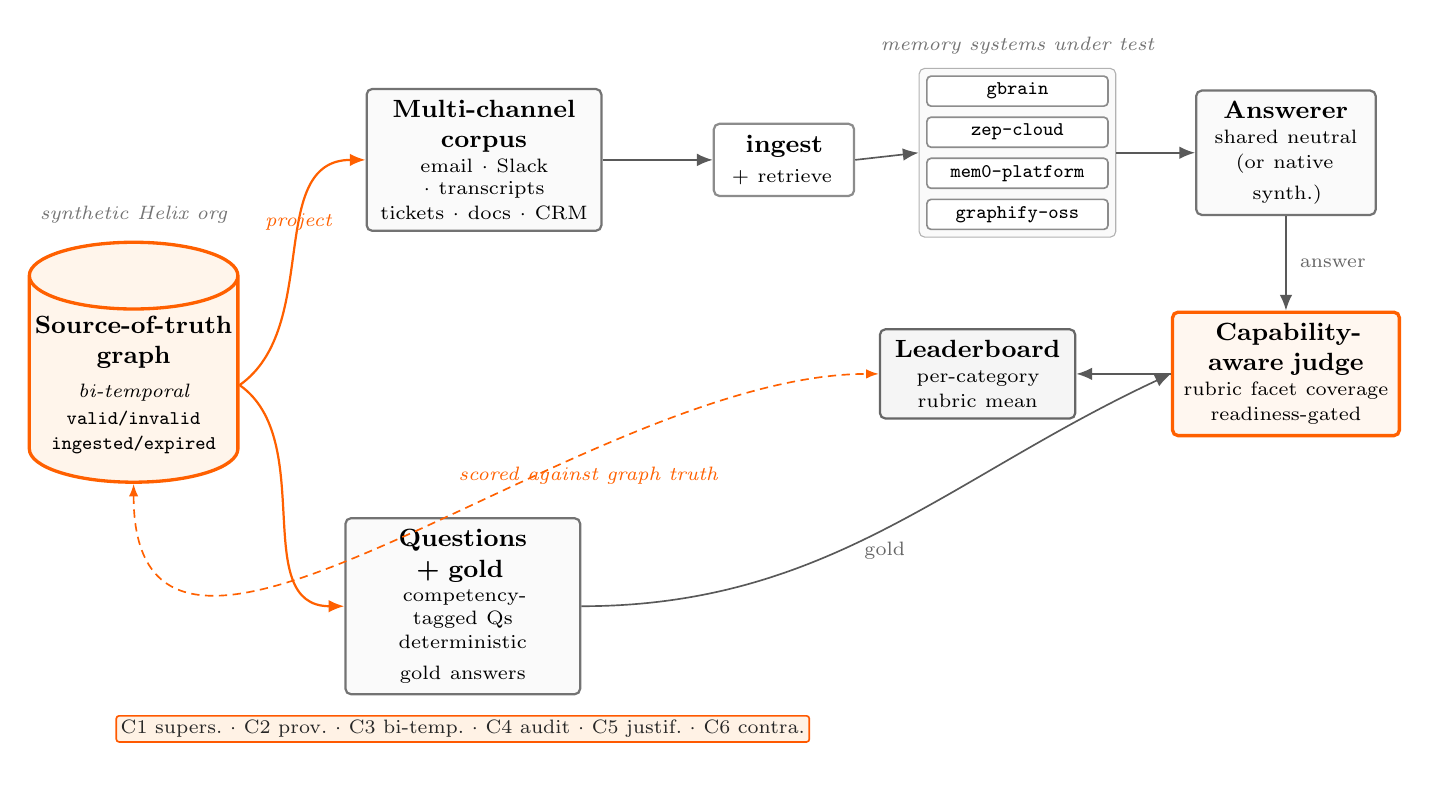
\begin{tikzpicture}[
    font=\small,
    node distance=6mm,
    accent/.style={orange!75!red},
    % --- the bi-temporal source-of-truth graph (origin) ---
    graph/.style={cylinder, shape border rotate=90, aspect=0.32, draw=orange!75!red,
                  very thick, fill=orange!8, minimum width=20mm, minimum height=15mm,
                  align=center, inner sep=2pt, text=black},
    % --- generic stage box ---
    box/.style={draw=black!55, thick, rounded corners=2pt, fill=black!2,
                align=center, inner sep=4pt, minimum height=9mm, text width=24mm},
    % --- system-under-test chip ---
    sys/.style={draw=black!45, semithick, rounded corners=1.5pt, fill=white,
                font=\scriptsize\ttfamily, inner sep=2.5pt, minimum width=23mm,
                align=center},
    % --- competency tag ---
    tag/.style={draw=orange!70!red, semithick, rounded corners=1pt, fill=orange!10,
                font=\scriptsize, inner sep=1.6pt, text=black!85},
    % --- judge / output emphasis ---
    judge/.style={draw=orange!75!red, very thick, rounded corners=2pt, fill=orange!6,
                  align=center, inner sep=4pt, minimum height=9mm, text width=26mm},
    board/.style={draw=black!60, thick, rounded corners=2pt, fill=black!4,
                  align=center, inner sep=4pt, minimum height=9mm, text width=22mm},
    flow/.style={-{Latex[length=2mm,width=1.6mm]}, black!65, semithick},
    proj/.style={-{Latex[length=2mm,width=1.6mm]}, orange!75!red, thick},
    scored/.style={{Latex[length=1.6mm]}-{Latex[length=1.6mm]}, densely dashed,
                   orange!75!red, semithick},
  ]

  % ---- ORIGIN: bi-temporal source-of-truth graph -------------------------
  \node[graph] (graph) {\textbf{Source-of-truth}\\\textbf{graph}\\[1pt]
        \scriptsize\itshape bi-temporal\\[-1pt]
        \scriptsize\ttfamily valid/invalid\\[-2pt]
        \scriptsize\ttfamily ingested/expired};
  \node[font=\scriptsize\itshape, text=black!55, above=1mm of graph]
        {synthetic Helix org};

  % ---- DUAL PROJECTION targets (the key idea) ----------------------------
  \node[box, above right=6mm and 16mm of graph, text width=27mm] (corpus)
        {\textbf{Multi-channel corpus}\\[1pt]
         \scriptsize email $\cdot$ Slack $\cdot$ transcripts\\[-2pt]
         \scriptsize tickets $\cdot$ docs $\cdot$ CRM};
  \node[box, below right=6mm and 16mm of graph, text width=27mm] (gold)
        {\textbf{Questions + gold}\\[1pt]
         \scriptsize competency-tagged Qs\\[-2pt]
         \scriptsize deterministic gold answers};

  % competency tags C1-C6 hanging under the questions
  \node[tag, below=2.5mm of gold] (tags)
        {C1 supers.\ $\cdot$ C2 prov.\ $\cdot$ C3 bi-temp.\ $\cdot$
         C4 audit $\cdot$ C5 justif.\ $\cdot$ C6 contra.};

  % projection arrows from the one graph (orange = "projected from graph")
  \draw[proj] (graph.east) to[out=35,in=180]
        node[pos=0.55, above=-0.5mm, accent, font=\scriptsize\itshape] {project}
        (corpus.west);
  \draw[proj] (graph.east) to[out=-35,in=180] (gold.west);

  % ---- SYSTEMS UNDER TEST -------------------------------------------------
  \node[box, right=14mm of corpus, text width=15mm, fill=white, draw=black!45]
        (ingest) {\textbf{ingest}\\\scriptsize+ retrieve};
  \node[sys, above right=2mm and 9mm of ingest] (s1) {gbrain};
  \node[sys, below=1.2mm of s1] (s2) {zep-cloud};
  \node[sys, below=1.2mm of s2] (s3) {mem0-platform};
  \node[sys, below=1.2mm of s3] (s4) {graphify-oss};
  \begin{scope}[on background layer]
    \node[draw=black!30, rounded corners=2pt, fill=black!2, fit=(s1)(s4),
          inner sep=2.5pt] (systems) {};
  \end{scope}
  \node[font=\scriptsize\itshape, text=black!55, above=0.5mm of systems]
        {memory systems under test};

  \draw[flow] (corpus.east) -- (ingest.west);
  \draw[flow] (ingest.east) -- (systems.west);

  % ---- ANSWERER -----------------------------------------------------------
  \node[box, right=10mm of systems, text width=20mm] (answerer)
        {\textbf{Answerer}\\[1pt]
         \scriptsize shared neutral\\[-2pt]
         \scriptsize (or native synth.)};
  \draw[flow] (systems.east) -- (answerer.west);

  % ---- JUDGE (capability-aware, rubric) ----------------------------------
  \node[judge, below=12mm of answerer] (judge)
        {\textbf{Capability-aware judge}\\[1pt]
         \scriptsize rubric facet coverage\\[-2pt]
         \scriptsize readiness-gated};
  \draw[flow] (answerer.south) -- node[right=0.5mm, font=\scriptsize, text=black!60]
        {answer} (judge.north);

  % ---- LEADERBOARD --------------------------------------------------------
  \node[board, left=12mm of judge] (board)
        {\textbf{Leaderboard}\\[1pt]
         \scriptsize per-category\\[-2pt]
         \scriptsize rubric mean};
  \draw[flow] (judge.west) -- (board.east);

  % gold answers feed the judge, and visibly trace back to the SAME graph
  \draw[flow] (gold.east) to[out=0,in=205]
        node[pos=0.5, below=0.3mm, font=\scriptsize, text=black!60] {gold}
        (judge.west);
  % the dashed "scored against" link: gold (graph-projected) <-> judged answer
  \draw[scored] (graph.south) to[out=-90,in=180]
        node[pos=0.7, below=0.5mm, accent, font=\scriptsize\itshape]
        {scored against graph truth} (board.west);

\end{tikzpicture}

% Keep the existing \caption{...}\label{fig:teaser}; do not caption inside here.
% =============================================================================
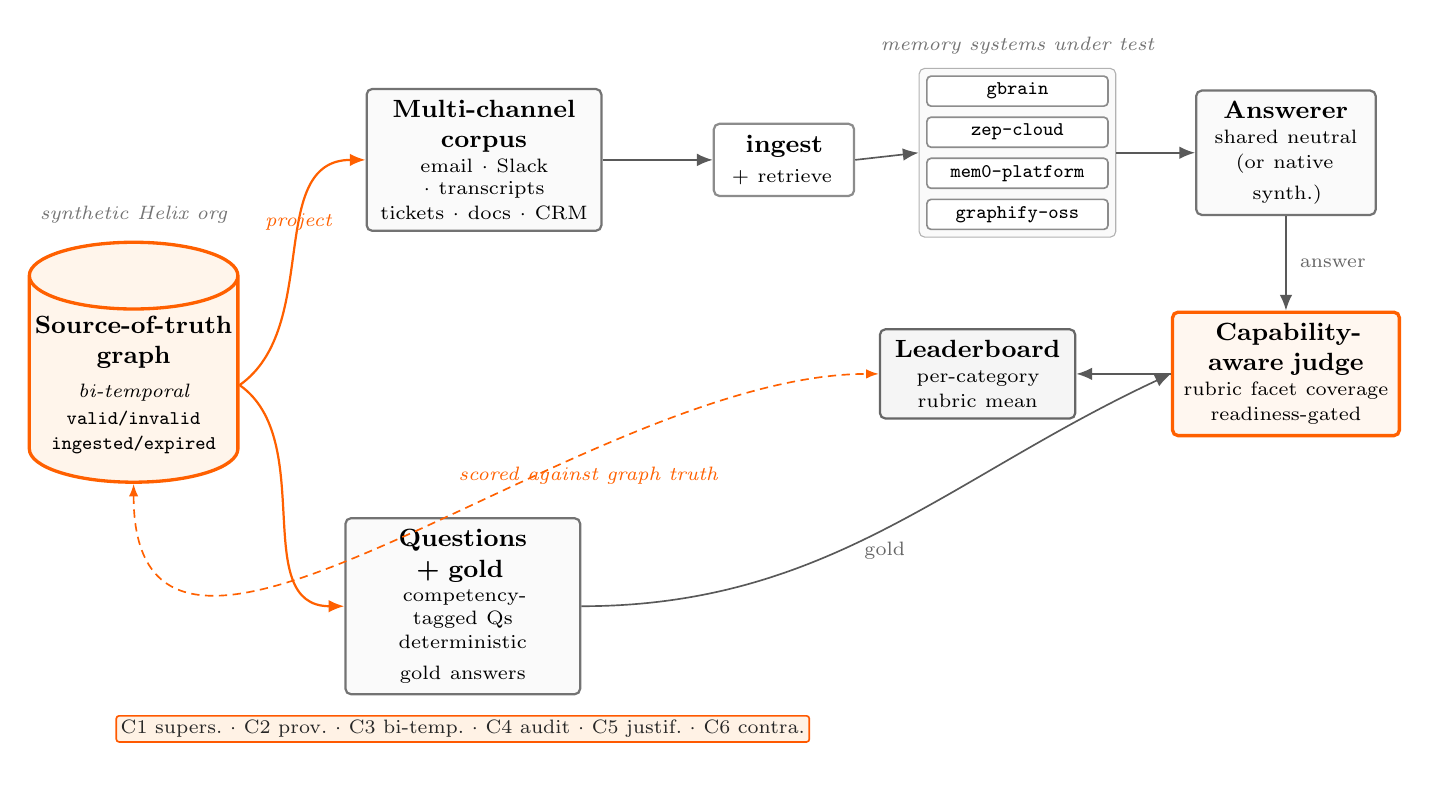
\begin{tikzpicture}[
    font=\small,
    node distance=6mm,
    accent/.style={orange!75!red},
    % --- the bi-temporal source-of-truth graph (origin) ---
    graph/.style={cylinder, shape border rotate=90, aspect=0.32, draw=orange!75!red,
                  very thick, fill=orange!8, minimum width=20mm, minimum height=15mm,
                  align=center, inner sep=2pt, text=black},
    % --- generic stage box ---
    box/.style={draw=black!55, thick, rounded corners=2pt, fill=black!2,
                align=center, inner sep=4pt, minimum height=9mm, text width=24mm},
    % --- system-under-test chip ---
    sys/.style={draw=black!45, semithick, rounded corners=1.5pt, fill=white,
                font=\scriptsize\ttfamily, inner sep=2.5pt, minimum width=23mm,
                align=center},
    % --- competency tag ---
    tag/.style={draw=orange!70!red, semithick, rounded corners=1pt, fill=orange!10,
                font=\scriptsize, inner sep=1.6pt, text=black!85},
    % --- judge / output emphasis ---
    judge/.style={draw=orange!75!red, very thick, rounded corners=2pt, fill=orange!6,
                  align=center, inner sep=4pt, minimum height=9mm, text width=26mm},
    board/.style={draw=black!60, thick, rounded corners=2pt, fill=black!4,
                  align=center, inner sep=4pt, minimum height=9mm, text width=22mm},
    flow/.style={-{Latex[length=2mm,width=1.6mm]}, black!65, semithick},
    proj/.style={-{Latex[length=2mm,width=1.6mm]}, orange!75!red, thick},
    scored/.style={{Latex[length=1.6mm]}-{Latex[length=1.6mm]}, densely dashed,
                   orange!75!red, semithick},
  ]

  % ---- ORIGIN: bi-temporal source-of-truth graph -------------------------
  \node[graph] (graph) {\textbf{Source-of-truth}\\\textbf{graph}\\[1pt]
        \scriptsize\itshape bi-temporal\\[-1pt]
        \scriptsize\ttfamily valid/invalid\\[-2pt]
        \scriptsize\ttfamily ingested/expired};
  \node[font=\scriptsize\itshape, text=black!55, above=1mm of graph]
        {synthetic Helix org};

  % ---- DUAL PROJECTION targets (the key idea) ----------------------------
  \node[box, above right=6mm and 16mm of graph, text width=27mm] (corpus)
        {\textbf{Multi-channel corpus}\\[1pt]
         \scriptsize email $\cdot$ Slack $\cdot$ transcripts\\[-2pt]
         \scriptsize tickets $\cdot$ docs $\cdot$ CRM};
  \node[box, below right=6mm and 16mm of graph, text width=27mm] (gold)
        {\textbf{Questions + gold}\\[1pt]
         \scriptsize competency-tagged Qs\\[-2pt]
         \scriptsize deterministic gold answers};

  % competency tags C1-C6 hanging under the questions
  \node[tag, below=2.5mm of gold] (tags)
        {C1 supers.\ $\cdot$ C2 prov.\ $\cdot$ C3 bi-temp.\ $\cdot$
         C4 audit $\cdot$ C5 justif.\ $\cdot$ C6 contra.};

  % projection arrows from the one graph (orange = "projected from graph")
  \draw[proj] (graph.east) to[out=35,in=180]
        node[pos=0.55, above=-0.5mm, accent, font=\scriptsize\itshape] {project}
        (corpus.west);
  \draw[proj] (graph.east) to[out=-35,in=180] (gold.west);

  % ---- SYSTEMS UNDER TEST -------------------------------------------------
  \node[box, right=14mm of corpus, text width=15mm, fill=white, draw=black!45]
        (ingest) {\textbf{ingest}\\\scriptsize+ retrieve};
  \node[sys, above right=2mm and 9mm of ingest] (s1) {gbrain};
  \node[sys, below=1.2mm of s1] (s2) {zep-cloud};
  \node[sys, below=1.2mm of s2] (s3) {mem0-platform};
  \node[sys, below=1.2mm of s3] (s4) {graphify-oss};
  \begin{scope}[on background layer]
    \node[draw=black!30, rounded corners=2pt, fill=black!2, fit=(s1)(s4),
          inner sep=2.5pt] (systems) {};
  \end{scope}
  \node[font=\scriptsize\itshape, text=black!55, above=0.5mm of systems]
        {memory systems under test};

  \draw[flow] (corpus.east) -- (ingest.west);
  \draw[flow] (ingest.east) -- (systems.west);

  % ---- ANSWERER -----------------------------------------------------------
  \node[box, right=10mm of systems, text width=20mm] (answerer)
        {\textbf{Answerer}\\[1pt]
         \scriptsize shared neutral\\[-2pt]
         \scriptsize (or native synth.)};
  \draw[flow] (systems.east) -- (answerer.west);

  % ---- JUDGE (capability-aware, rubric) ----------------------------------
  \node[judge, below=12mm of answerer] (judge)
        {\textbf{Capability-aware judge}\\[1pt]
         \scriptsize rubric facet coverage\\[-2pt]
         \scriptsize readiness-gated};
  \draw[flow] (answerer.south) -- node[right=0.5mm, font=\scriptsize, text=black!60]
        {answer} (judge.north);

  % ---- LEADERBOARD --------------------------------------------------------
  \node[board, left=12mm of judge] (board)
        {\textbf{Leaderboard}\\[1pt]
         \scriptsize per-category\\[-2pt]
         \scriptsize rubric mean};
  \draw[flow] (judge.west) -- (board.east);

  % gold answers feed the judge, and visibly trace back to the SAME graph
  \draw[flow] (gold.east) to[out=0,in=205]
        node[pos=0.5, below=0.3mm, font=\scriptsize, text=black!60] {gold}
        (judge.west);
  % the dashed "scored against" link: gold (graph-projected) <-> judged answer
  \draw[scored] (graph.south) to[out=-90,in=180]
        node[pos=0.7, below=0.5mm, accent, font=\scriptsize\itshape]
        {scored against graph truth} (board.west);

\end{tikzpicture}
}
  \caption{\textbf{The \bench{} evaluation pipeline.} A multi-channel, multi-author
    synthetic organizational corpus (email, Slack, meeting transcripts, tickets,
    wikis, CRM) is ingested by each memory system. Competency-tagged questions
    (the six small/medium-tier competencies: supersession, decision provenance,
    bi-temporal, audit replay, justification chains, contradiction) are answered
    through a shared answerer
    and scored by a fixed LLM-as-judge rubric, with a readiness gate ensuring hosted
    asynchronous systems are fully ingested before querying. The strongest public
    system answers only $\sim$$39\%$ of the task.}
  \label{fig:teaser}
\end{figure}


% Compact leaderboard teaser (tab:leaderboard) --- a [t] float so the headline
% result surfaces on the first page-turn. Full per-category table is in Experiments.
%==============================================================================
% LEADERBOARD (compact, intro-adjacent) --- headline result up front.
%
% Owned by the introduction restructure pass. The orchestrator wires the
% \input order in main.tex (this file is \input'd just after the intro prose,
% before/with the teaser). Numbers are the top-level tier means from
% tab:main-results (results.tex, sec:exp:main): the Mean column only. The full
% per-category breakdown stays in Table~\ref{tab:main-results} (Experiments).
%
% Cross-refs OUT: \ref{tab:categories} (C-taxonomy), \ref{sec:experiments}
% (full table + analysis). Cross-refs IN: \ref{tab:leaderboard} from
% introduction.tex (headline para + contributions) and abstract/results.
%==============================================================================
\begin{table}[t]
  \centering
  \caption{\textbf{\bench{} leaderboard: top-level rubric score by tier
    (higher is better, $[0,1]$).} Mean rubric-weighted score over all questions
    in a tier, for the four publicly available memory systems, ordered by
    medium-tier mean. No system is close to solving the task: the strongest
    public system, \texttt{gbrain}, reaches only $0.394$ (small) and $0.428$
    (medium), and the small-tier ordering does not survive the move to the
    medium tier (\texttt{mem0-platform} and \texttt{zep-cloud} swap rank). The
    full per-category breakdown over the six \bench{} competencies (C1--C6;
    Table~\ref{tab:categories}) is in Table~\ref{tab:main-results}
    (\S\ref{sec:experiments}). Single seed; see \S\ref{sec:exp:setup} for the
    variance caveat.}
  \label{tab:leaderboard}
  \small
  \begin{tabular}{l S[table-format=1.3] S[table-format=1.3]}
    \toprule
    {System} & {Small mean} & {Medium mean} \\
    \midrule
    \texttt{gbrain}        & \bfseries 0.394 & \bfseries 0.428 \\
    \texttt{mem0-platform} & 0.221 & 0.303 \\
    \texttt{zep-cloud}     & 0.252 & 0.213 \\
    \texttt{graphify-oss}  & 0.206 & 0.142 \\
    \bottomrule
  \end{tabular}
  \par\smallskip
  {\footnotesize Small tier: 11 questions, 121 artifacts ($\approx$60K tokens).
  Medium tier: 73 questions, 443 artifacts ($\approx$200K tokens). Bold marks
  the best value per column.}
\end{table}


%==============================================================================
% 2. RELATED WORK
%==============================================================================
%==============================================================================
% 2. RELATED WORK
%==============================================================================
% Drafted from paper/.research/landscape.md (refreshed 2026-05-29) and design.md.
% Cite keys used (all defined in refs.bib):
%   gbrain, zep_graphiti_2025, mem0_2024, graphify_oss            (systems)
%   maharana2024locomo, wu2024longmemeval, beam2025,
%   hu2025memoryagentbench, memorybench2025                        (benchmarks)
%   gebru2021datasheets, croissant2024   (D&B methodology -- now cited in design.tex
%                                          / main.tex; methodology subsection relocated)
% Scope discipline: the public field evaluated here is EXACTLY four systems
% (gbrain, zep-cloud, mem0-platform, graphify-oss). No authors'-own system is
% referenced anywhere.
%==============================================================================
\section{Related Work}
\label{sec:related}

\bench{} sits at the intersection of three lines of work: the agent-memory
systems it evaluates, the benchmarks that currently measure them, and the
broader literature on long-horizon and temporal reasoning. We close the section
by situating \bench{} against existing benchmarks on the axes that distinguish
organizational memory (Table~\ref{tab:bench-comparison}).

\subsection{AI Agent Memory Systems}
\label{sec:related:systems}

A memory system gives an agent persistent state beyond its context window: it
ingests a stream of text, decides what to store and in what representation, and
retrieves the relevant fragments when a later query arrives. The four publicly
available systems we evaluate span the dominant architectural families and make
sharply different design bets, which is precisely why a benchmark that exercises
them under a single harness is informative.

\textbf{gbrain} is an open hybrid-retrieval system~\citep{gbrain} that combines
lexical (BM25), dense vector, and graph-based retrieval over an extracted store,
then fuses the three signals at query time. The hybrid design is intended to
recover both surface lexical matches and semantically paraphrased evidence while
using graph structure to follow relations between entities.

\textbf{Zep}, built on the Graphiti engine~\citep{zep_graphiti_2025}, maintains a
\emph{temporal knowledge graph}: ingested text is distilled into entities and
relations whose edges carry validity intervals, so the graph can in principle be
queried for the state of the world as of a given date and can represent facts that
were later invalidated. Of the four systems it is architecturally closest to the
bi-temporal structure \bench{} probes, which makes its performance a useful test
of whether a temporal-graph representation, on its own, suffices for
organizational-scale questions.

\textbf{Mem0}~\citep{mem0_2024} follows an extract-and-store paradigm aimed at
production deployment: an extraction step converts incoming messages into compact
natural-language memories, with subsequent operations to add, update, or
invalidate them as new information arrives. The representation is optimized for
scalable low-latency retrieval of salient personal facts rather than for
reconstructing a multi-author audit trail.

\textbf{graphify}~\citep{graphify_oss} is an open-source, embedding-free library
that stores memories as a graph and retrieves by explicit BFS/DFS traversal rather
than by vector similarity. By avoiding dense embeddings it removes one source of
opaque approximation, but it also forgoes the soft semantic matching the other
systems rely on, trading recall on paraphrased evidence for transparent, traversal-based
retrieval.

{\sloppy These systems are evaluated head-to-head under a uniform protocol, each
on its vendor-recommended configuration, in Section~\ref{sec:experiments}.\par}

\subsection{Existing Memory Benchmarks}
\label{sec:related:benchmarks}

The benchmarks that currently define progress on agent memory share one structural
assumption: memory is a \emph{single narrator's} history, possibly very long.

\textbf{LoCoMo}~\citep{maharana2024locomo} evaluates very-long-term \emph{two-party}
dialogue grounded in speaker personas and temporally ordered event graphs
(Table~\ref{tab:bench-comparison}). Its temporal-QA category touches evolving facts,
but supersession with explicit attribution is not a labeled task, and the corpus is
a single shared dyadic narrative rather than a multi-author organization. Top
systems now cluster between roughly 83\% and 93\%; tellingly, the numbers are also
\emph{disputed}, with different evaluators reporting materially different scores for
the same systems, which is itself an argument for a neutral, fixed-harness
benchmark.

\textbf{LongMemEval}~\citep{wu2024longmemeval} measures five memory abilities over
scalable user-assistant chat. Crucially, its knowledge-update and temporal
categories operate \emph{within one user's own stated facts}: there is no
multi-author corpus, no channel heterogeneity, and no role structure. Leading
systems now exceed 83\%.

\textbf{BEAM}~\citep{beam2025} pushes the \emph{volume} frontier, with ten memory
tasks (including knowledge update, contradiction resolution, event ordering, and
abstention) over coherent \emph{single-narrator} conversations generated up to 10M
tokens across two tracks (1M and 10M). At extreme scale it is not saturated:
reported best accuracy is about 64\% at 1M tokens and about 49\% at 10M. But the
challenge it poses is one of how \emph{much} a single narrator said, not of
\emph{who} said what across an organization; it varies length, not source
heterogeneity.

\textbf{MemoryAgentBench}~\citep{hu2025memoryagentbench} shifts toward agentic,
incremental multi-turn interaction over chunked inputs, a meaningful move beyond
static QA, but it still models one agent processing one input stream. Related
continual-learning and memory-hallucination benchmarks, including
MemoryBench~\citep{memorybench2025}, share the same single-user, personal-scale
framing and are not analyzed individually here.

The common thread is that near-saturation on LoCoMo and LongMemEval does not show
that memory is solved; it shows the benchmarks have stopped measuring the hard
part. Table~\ref{tab:bench-comparison} makes the gap concrete on the decisive
axes: \emph{modality}, where prior work is two-party, single-narrator, or
user--assistant dialogue while \bench{} is a multi-channel organizational corpus
authored by many distinct people; and \emph{scale}, where prior work grows one
narrator's history in \emph{length} (to ${\sim}1$M and 10M tokens) while \bench{}
instead grows \emph{breadth}---more authors, channels, and a multi-year timeline.
The remaining axes are where prior work is uniformly weak: none varies author
count (\emph{multi-source}), and although several include knowledge-update QA, none
treats \emph{supersession}---a fact invalidated and replaced, carrying an
attributed reason and date---as a first-class, labeled reasoning category.

\subsection{Long-Horizon and Temporal Reasoning}
\label{sec:related:temporal}

Beyond memory systems specifically, \bench{} draws on two strands of work on
temporal reasoning in language. The first concerns \emph{long-context} models and
retrieval-augmented generation, where a recurring finding is that the ability to
\emph{attend} to a long input is not the ability to \emph{reason} over information
distributed across it. The second concerns \emph{temporal} structure:
distinguishing valid-time (when a fact held in the world) from ingest-time (when it
was recorded), and reconstructing knowledge as of a past date. \bench{} makes this
structure first-class through the bi-temporal source-of-truth graph described in
\S\ref{sec:design}, and it is the dimension on which we observe the sharpest
degradation across all evaluated systems.

% COMPARISON TABLE: OrgMemBench vs existing benchmarks on the axes that define
% organizational memory. booktabs, no vertical rules (guide 1.6). SOTA / scale
% facts from landscape.md; OrgMemBench medium leaderboard is planned (see note).
\begin{table}[t]
  \centering
  \caption{\textbf{\bench{} versus existing memory benchmarks.} To our knowledge
    the first benchmark to target multi-source, multi-author organizational memory
    with bi-temporal supersession as a labeled reasoning category. The axes are
    walked through in the text (\S\ref{sec:related:benchmarks}).}
  \label{tab:bench-comparison}
  \small
  \setlength{\tabcolsep}{4pt}
  \begin{tabular}{@{}l p{2.5cm} p{2.5cm} l c c c@{}}
    \toprule
    & & & Temporal & Multi- & Super- & Public \\
    Benchmark & Modality & Scale & span & source & session & leaderboard \\
    \midrule
    LoCoMo
      & Dyadic dialogue + image
      & $\sim$9K tok/conv (50)
      & Up to 35 sess.
      & No
      & Partial
      & Informal \\
    LongMemEval
      & User--assistant chat
      & 128K\,$\rightarrow\sim$1M tok
      & Multi-session
      & No
      & Yes
      & Yes \\
    BEAM
      & Single-narrator dialogue
      & Up to 10M tok/conv
      & $\sim$1 year
      & No
      & Yes
      & Yes \\
    \midrule
    \bench{} (ours)
      & Multi-channel org.\ corpus
      & $\sim$63K (S) / ${>}200$K (M) tok
      & Multi-year
      & Yes
      & Yes
      & Planned \\
    \bottomrule
  \end{tabular}
  \par\smallskip
  {\footnotesize ``Partial'' for LoCoMo reflects its temporal-QA category, which
  touches evolving facts but does not label supersession with attribution. Token
  scales are approximate; \bench{} figures are plain-text corpus totals.}
\end{table}


%==============================================================================
% 3. ORGMEMBENCH DESIGN  (the core contribution)
%    design.tex opens \section{\bench{} Design}; generation.tex continues it
%    with the data-generation and manual-corrections subsections.
%==============================================================================
%==============================================================================
% 3. OrgMemBench Design  (the core contribution)
%==============================================================================
\section{\bench{} Design}
\label{sec:design}

\subsection{Overview: Goals and Scope}
\label{sec:design:overview}

\bench{} is designed to measure one capability that existing benchmarks do not
reach: an agent's ability to answer everyday organizational questions over a
multi-source, multi-author, multi-year record of work. Concretely, the target
queries are the kind a person routinely routes to an assistant with access to
the company's history---``who owns the Acme relationship, and where was that
established?'', ``what did engineering decide about the migration last quarter,
and has that changed?''
Answering these requires stitching evidence across channels (email, Slack,
meeting transcripts, tickets, documents, CRM entries), across people whose roles
and seniority shift over time, and across time itself---including facts that
were later superseded, corrected, held in unresolved contradiction, or never
written down explicitly as a rule. The benchmark is built around four design
principles that follow from this target: ground truth is projected
deterministically from a known source-of-truth graph rather than read back out
of free text; the temporal model is bi-temporal so that ``what was true then''
can be separated from ``what the organization recorded, and when''; scoring is
rubric-based facet coverage rather than exact match, so that multiple correct
phrasings earn credit while omissions are penalized deterministically; and the
harness is \emph{capability-aware}, reporting a category as not-applicable for a
system whose design cannot in principle answer it (for example, an as-of-date
temporal query posed to a system with no temporal model) rather than silently
scoring it zero.

It is equally important to state what \bench{} does \emph{not} test. It is not a
conversational or personal-memory benchmark (the regime LoCoMo, LongMemEval, and
BEAM cover); the full scope boundaries are enumerated in
\S\ref{app:construction}.

\subsection{The Helix Organization and the Bi-temporal Model}
\label{sec:design:helix}

The seed organization is \textbf{Helix Logistics}, a small-to-mid-size
SaaS/freight-tech company instantiated with a coherent multi-year narrative arc:
founded in 2020 by Maya Patel and Daniel Kim, it ships its API and pivots toward
mid-market, weathers a customer escalation and reorganization, and overhauls its
documentation, across a dated 2020--2026 timeline. A fixed company skeleton pins
the founding year, founders, per-year arcs, documentation-discipline eras,
product lines, and a tooling timeline with explicit replacements (for example,
Salesforce replaces HubSpot and Confluence replaces Notion in successive years);
those replacements are not decoration---they seed the temporal and supersession
structure that the hard question categories then probe. The full company
skeleton is enumerated in \S\ref{app:construction}.

The substrate that makes this possible is a \textbf{bi-temporal}
source-of-truth graph. Every event and fact carries four timestamps:
\texttt{valid\_at} (when it became true in the world), \texttt{invalid\_at}
(when it stopped being true), \texttt{ingested\_at} (when the organization
recorded it), and \texttt{expired\_at} (when that record was retracted or
corrected). Two timelines therefore coexist---\emph{valid time} (the world) and
\emph{transaction time} (the record)---and a question can interrogate either or
both. Facts are \textbf{invalidated, never deleted}, which preserves a no-loss
audit trail: the prior state of any fact remains recoverable alongside its
replacement. When one fact replaces another, a \textbf{supersession link}
connects the old fact to the new one together with an explicit \emph{reason}, so
the change is not merely detectable but explainable. Finally, the model supports
\textbf{\texttt{as\_of} date-travel}: a query can reconstruct what the
organization believed on a specified past date, which is distinct from what is
true now. This structure licenses the C1/C3/C4 categories below.

\subsection{Question Taxonomy}
\label{sec:design:taxonomy}
\label{sec:design:questions}

{\sloppy
Each tier ships a versioned question set spanning six structured categories
(C1--C6; Table~\ref{tab:categories}), each isolating a distinct reasoning pattern
and pinned to the facets a correct answer must recover. A seventh,
\textsc{Emergent}, category (reconstructing a de-facto pattern never written down
as an explicit rule) is deferred to the large tier and is out of scope here. The
small tier poses $11$ questions over a $121$-artifact corpus ($\approx$60K
tokens); the medium tier poses $73$ questions over $443$ artifacts
($\approx$200K tokens)---the unit of scale being the corpus a system must ingest
and retrieve over, not the question count alone. Question counts per category and
tier are given in Appendix~\ref{app:construction}
(Table~\ref{tab:design:counts}).
\par}

\begin{table}[t]
  \centering
  \caption{\textbf{Category definitions.} The six structured categories
    evaluated at the small and medium tiers. A seventh category, emergent
    pattern, is evaluated only at the large tier and above and is out of scope
    here.}
  \label{tab:categories}
  \begin{tabular}{l l p{0.46\textwidth}}
    \toprule
    Code & Name & What it tests \\
    \midrule
    C1 & Supersession        & The current value of a fact plus what it
                               replaced, when, and why. Example: \emph{``What is
                               the data-retention policy now, what did it
                               replace, and what drove the change?''} \\
    C2 & Decision provenance & Who decided, when, what alternatives were
                               weighed, and the deciding rationale. Example:
                               \emph{``Who chose the cloud-native migration and
                               what options were rejected?''} \\
    C3 & Bi-temporal (as-of) & What the organization believed AS OF a past date,
                               distinct from now. Example: \emph{``What would the
                               answer have been on 2022-01-15?''} \\
    C4 & Audit replay        & Reconstruct the knowledge state at a past date and
                               flag what has since changed. \\
    C5 & Justification chain & Enumerate the evidence supporting a conclusion and
                               classify each as direct testimony vs. inference. \\
    C6 & Contradiction       & Detect that two artifacts conflict; report both
                               sides and whether it was resolved. \\
    \bottomrule
  \end{tabular}
\end{table}

The ground-truth and rubric field schemas, the $72$-persona library and
document-genre taxonomy, and the artifact counts behind these question sets are
detailed in Appendix~\ref{app:construction}.

\subsection{Synthetic Generation}
\label{sec:design:why-synthetic}
\label{sec:generation}
\label{sec:design:generation}

The data is synthetic by deliberate design: a freshly generated fictional
organization cannot appear in any system's pretraining data or retrieval cache, so
a high score cannot be explained by memorization---a stronger guarantee than
post-hoc $n$-gram decontamination, which can only estimate leakage that has
already occurred (the further reasons of control and privacy are developed in
Appendix~\ref{app:construction}). Ground-truth labels are deterministic
projections of the source-of-truth graph rather than free-text recall, which
sharply limits label ambiguity but does not remove the single-model circularity
inherent in one model writing the artifacts, phrasing the questions, and running
the self-consistency check; following \citet{gebru2021datasheets} we document
this rather than obscure it (in a full datasheet, Appendix~\ref{app:datasheet}),
and a cross-model validation pass is planned. We accompany the release with
Croissant metadata~\citep{croissant2024} so the dataset is machine-discoverable
and ML-ready. The \texttt{helix-corpus} generation tooling (a single local
\texttt{gpt-oss:20b} model served via Ollama), the full Stage~A--F pipeline, and
the logged, reversible three-wave manual audit that reconciled shipped files with
the graph without altering the answer key are detailed in
Appendix~\ref{app:construction}; the audit log and its six defect classes in
Appendix~\ref{app:annotation}.

%==============================================================================
% Synthetic Data Generation --- GUTTED to 0pp.
%
% This standalone section no longer carries body content. Per the body-trim plan:
%
%   * The label-bearing body residue (the short \subsection{Synthetic Data
%     Generation} carrying \label{sec:generation} and \label{sec:design:generation})
%     is folded into the TAIL OF THE DESIGN SECTION (sections/design.tex), which
%     OWNS and authors it. Those two labels live there now and still resolve the
%     refs in limitations.tex (sec:design:generation) and main.tex (sec:design:
%     generation). Do NOT re-add them here, or LaTeX will report multiply-defined
%     labels.
%
%   * The full Stage~A--F pipeline, genre taxonomy, documentation-discipline eras,
%     and the circularity structural-defenses enumeration are relocated to the
%     appendix "Benchmark Construction Detail" (sections/app_construction_detail.tex,
%     \label{app:construction}, owned by the design agent).
%
%   * The Manual Corrections and Audit Trail subsection, the six per-defect
%     autopsies, and the corrections-closer are relocated to the appendix
%     "Annotation and Audit Process (extended)"
%     (sections/app_annotation_audit_detail.tex), which carries the migrated
%     \label{sec:generation-corrections} (referenced by main.tex:253 and the
%     datasheet's preprocessing/cleaning subsection).
%
% This file is still \input from main.tex immediately after sections/design; it is
% intentionally empty of typeset content so its body contribution is 0pp.
%==============================================================================


%==============================================================================
% 4. EXPERIMENTS  (baselines.tex is now the opening \subsection; results.tex
%    supplies the remaining subsections)
%==============================================================================
\section{Experiments}
\label{sec:experiments}
%==============================================================================
% 4. BASELINE SYSTEMS
%   Demoted to a \subsection and relocated to the front of Experiments; the
%   enclosing \section{Experiments} and the \input ordering are wired in
%   main.tex. Architecture prose lives in \S\ref{sec:related:systems} and
%   Table~\ref{tab:baseline-config}; the answerer/judge policy lives in
%   \S\ref{sec:exp:setup}. This file keeps only eval-relevant deltas + the
%   config table.
%==============================================================================
\subsection{Baseline Systems}
\label{sec:baselines}

We evaluate the four memory systems that are publicly available and can be run
end-to-end against an external corpus: \texttt{gbrain}, \texttt{zep-cloud}
(Zep/Graphiti), \texttt{mem0-platform} (Mem0 hosted), and \texttt{graphify-oss}.
Their architectures are described in \S\ref{sec:related:systems} and summarized
in Table~\ref{tab:baseline-config}; here we record only the choices that bear on
the evaluation---version pin, native-versus-shared answerer, ingest mode and
readiness drain, and the single mechanism that explains each system's score.
Scoring and answer synthesis are held constant across baselines per the answerer
policy in \S\ref{sec:exp:setup}. Full pins, drain recipes, and the
controlled-extractor probe are in Appendix~\ref{app:hyperparams}.

\paragraph{\texttt{gbrain} (\texttt{0.41.6.0}).}
Evaluated end-to-end with its native \texttt{think} synthesizer per the answerer
policy (\S\ref{sec:exp:setup}); ingestion is synchronous, so no readiness drain
is required.

\paragraph{\texttt{zep-cloud} (\texttt{3.22.0}).}
Run on the FREE plan~\citep{zep_graphiti_2025}; both its extractor and embeddings
are hosted and undisclosed, so they are part of the system under test rather than
parameters we control. Retrieved edges are routed through the shared neutral
answerer (it has no native one), and because ingestion is asynchronous a
probe-edge readiness drain (1800\,s) precedes querying.

\paragraph{\texttt{mem0-platform} (\texttt{2.0.2}).}
Run on the FREE plan~\citep{mem0_2024}; the shipped product uses an
\emph{undisclosed, non-configurable server-side extractor} (not Sonnet), so the
extractor is fixed by the vendor and evaluated as-is---the principal explanation
for its result. Results are routed through the shared neutral answerer, and as
with \texttt{zep-cloud} the asynchronous ingest demands a probe-search readiness
drain (900\,s; the choice of drain is itself a methodological finding,
\S\ref{sec:exp:readiness}).

\paragraph{\texttt{graphify-oss} (\texttt{0.8.20}).}
Extraction uses an LLM whose upstream-hardcoded default is Claude Sonnet~4.6,
matching our cross-system model; retrieved subgraphs go through the shared neutral
answerer; ingestion is synchronous with no drain. Its extraction is coarse and
document-granular---roughly \emph{one node per artifact}---the observation we
return to in the analysis.

\begin{table}[t]
  \centering
  \caption{\textbf{Baseline system configurations.} All systems are evaluated with
    the same Claude Sonnet~4.6 judge (extended thinking) and, except for
    \texttt{gbrain} (which uses its native \texttt{think} synthesizer), the same
    Claude Sonnet~4.6 neutral answerer. ``Extractor / synth.\ LLM'' is the model
    used for the memory-side processing under our control; ``hosted'' marks a
    component that is server-side and undisclosed. Top-$K=10$ wherever
    configurable. The bottom row is a controlled-extractor \emph{probe}, not the
    shipped product, and appears only in the appendix.}
  \label{tab:baseline-config}
  \small
  \resizebox{\textwidth}{!}{%
  \begin{tabular}{@{}llllll@{}}
    \toprule
    System & Version & Memory model & Extractor / synth.\ LLM & Embeddings & Ingest / readiness gate \\
    \midrule
    \texttt{gbrain}
      & \texttt{0.41.6.0}
      & hybrid BM25+vector+graph
      & Sonnet 4.6 (native \texttt{think})
      & ZeroEntropy \texttt{zembed-1}
      & sync; no drain \\
    \texttt{zep-cloud}
      & \texttt{3.22.0}
      & bi-temporal knowledge graph
      & hosted (undisclosed)
      & hosted (undisclosed)
      & async; probe-edge drain, 1800\,s \\
    \texttt{mem0-platform}
      & \texttt{2.0.2}
      & extracted memories + vector
      & hosted (undisclosed)
      & hosted (undisclosed)
      & async; probe-search drain, 900\,s \\
    \texttt{graphify-oss}
      & \texttt{0.8.20}
      & keyword-BFS graph
      & Sonnet 4.6 (upstream default)
      & none (pure BFS/DFS)
      & sync; no drain \\
    \midrule
    \textit{probe:} Mem0 OSS
      & \texttt{2.0.2}
      & extracted memories + vector
      & Sonnet 4.6 (controlled)
      & \texttt{text-embedding-3-small}
      & sync; no drain \\
    \bottomrule
  \end{tabular}%
  }
\end{table}

%==============================================================================
% Experiments, Results, and Analysis
%
% Drop-in body for Section 5 (Experiments). The enclosing \section{Experiments}
% and \label{sec:experiments} live in main.tex; this file supplies the
% condensed body subsections. All numbers are the verified means/per-category
% scores read off results/<system>/helix-{small,medium}.json and cross-checked
% against the ground-truth anchors. Public field = four systems (gbrain,
% zep-cloud, mem0-platform, graphify-oss); the only medium-tier run completed to
% date is gbrain. Per-system autopsies, the gbrain mechanism subsection, the full
% readiness case write-ups, per-run dollar figures, and judge token detail are in
% Appendix~\ref{app:extended} (Extended Results).
%==============================================================================

\subsection{Metrics and Setup}
\label{sec:exp:metrics}

\bench{} scores each answer with a \emph{rubric-weighted} judgment in $[0,1]$
rather than exact match. Every question ships with a weighted rubric (Stage~E,
\S\ref{sec:design:questions}): a small set of sub-criteria---typically the
specific fact, the date or time qualifier, the supersession or contradiction
relation, and the justification chain---each with an explicit weight. An answer
earns the weighted fraction of sub-criteria it satisfies, so partial credit
reflects \emph{which} part of an organizationally grounded answer a system got
right. The headline metric is the mean of this rubric score over the questions
in a tier. We report exact match only as a secondary diagnostic: it is
effectively zero across the board, because correct answers are multi-clause
statements no system reproduces verbatim, which is exactly why a sub-point rubric
is the appropriate instrument. An LLM judge with extended thinking scores each
answer against the per-sub-criterion rubric, awarding each sub-point
independently before summing, under the same configuration for every system
(token budgets, temperature, and output caps in Appendix~\ref{app:extended}).

The judge also labels each non-perfect answer with one of five mutually exclusive
failure modes---\texttt{retrieval\_miss}, \texttt{hallucination},
\texttt{wrong\_synthesis}, \texttt{wrong\_abstain}, and \texttt{none}---which lets
us separate \emph{retrieval} failures from \emph{reasoning} failures, a
distinction the scaling analysis below turns on.

\paragraph{Setup and answerer policy.}\label{sec:exp:setup}
Each system is evaluated in isolation: the tier corpus is ingested into a
\emph{fresh} store (scope isolated per tier), the system is driven through a
readiness gate (\S\ref{sec:exp:readiness}), and the tier's questions are then
issued and scored; hosted systems run over their public APIs and self-hosted
systems in pinned Docker images (pins in \S\ref{sec:baselines}/Appendix~\ref{app:hyperparams}).
Retrieval and answer synthesis are decoupled: a system that ships its own
synthesizer is run end-to-end with it (\texttt{gbrain} via native \texttt{think}),
the artifact a user would deploy, while retrieval-only systems
(\texttt{zep-cloud}, \texttt{mem0-platform}, \texttt{graphify-oss}) share one
fixed neutral answerer (Claude Sonnet~4.6) so differences reflect the memory
layer; top-$K=10$ wherever configurable.

\paragraph{Cost.}
End-to-end cost is $\approx$\$0.02--\$0.04 per question, dominated by the judge
and answerer; \texttt{graphify-oss}'s server-side Sonnet extraction dominates its
all-in cost ($\approx$\$0.13 per question at medium), with the full breakdown and
the \texttt{cost\_per\_query\_usd} metering caveat in
Appendix~\ref{app:extended}.

\paragraph{Statistical caveat (stated up front).}
These are \textbf{single-seed} results over \textbf{small} question sets (11
small, 73 medium), so we attach no confidence intervals and treat sub-$0.1$
between-system gaps as indicative rather than significant. The full treatment of
this variance---including the replication numbers---is in \S\ref{sec:limitations},
the body home for those figures.

\subsection{Main Results}
\label{sec:exp:main}

Table~\ref{tab:main-results} reports the headline rubric means. The central
finding is not that one system wins: it is that \textbf{organizational-scale
memory is unsolved}. The strongest currently-available public system,
\texttt{gbrain}, reaches only $0.394$ on the small tier and $0.428$ on the
medium tier; across both tiers the rest of the public field clusters between
$0.142$ and $0.303$. There is large headroom on every tier and in every
category, and the spread between the best public system and the rest, while
clear, is itself modest relative to the gap to a competent answer. We
deliberately frame \texttt{gbrain} as the strongest \emph{currently-available
public} system rather than as a solution: a $0.39$ ceiling on a benchmark whose
questions a human analyst with access to the corpus could largely answer is the
paper's motivating result, not a leaderboard victory. ``Leads'' is not
``solves'': \texttt{gbrain} scores $0.000$ on small-tier contradiction (C6) and
$0.122$ on bi-temporal (C3), and its $0.394$/$0.428$ means leave roughly
six-tenths of the achievable rubric credit on the table. The headline of the
benchmark is this remaining headroom, not the identity of the front-runner.

\begin{table}[t]
  \centering
  \caption{\textbf{End-to-end results on \bench{}: mean rubric score and
    per-category breakdown (higher is better).} A single consolidated view of
    both tiers. Top panel: the four public memory systems on the small tier
    (11 questions, 121 artifacts). Bottom panel: the same four on the medium tier
    (73 questions, 443 artifacts). Category columns abbreviate the
    six \bench{} categories (full definitions in Table~\ref{tab:categories}):
    Supers.~=~supersession (C1), Prov.~=~decision provenance (C2),
    Bi-temp.~=~bi-temporal as-of (C3), Audit~=~audit replay (C4),
    Justif.~=~justification chain (C5), Contra.~=~contradiction (C6). Best
    value per column within each tier in bold. Single seed; see \S\ref{sec:exp:setup}
    for the variance caveat. A controlled-extractor probe (\texttt{mem0} OSS +
    Sonnet, not a shipped product; Appendix~\ref{app:extended}) scores a $0.479$
    small-tier mean.}
  \label{tab:main-results}
  \begin{tabular}{l S[table-format=1.3]
      S[table-format=1.3] S[table-format=1.3] S[table-format=1.3]
      S[table-format=1.3] S[table-format=1.3] S[table-format=1.3]}
    \toprule
    {System} & {Mean} & {Supers.} & {Prov.} & {Bi-temp.} & {Audit} & {Justif.} & {Contra.} \\
    \midrule
    \multicolumn{8}{l}{\emph{Small tier} --- 11 questions, 121 artifacts ($\approx$60K tokens)} \\
    \texttt{gbrain}        & \bfseries 0.394 & \bfseries 0.675 & \bfseries 0.762 & 0.122 & \bfseries 0.533 & \bfseries 0.411 & 0.000 \\
    \texttt{zep-cloud}     & 0.252 & 0.525 & 0.625 & 0.172 & 0.000 & 0.117 & \bfseries 0.133 \\
    \texttt{mem0-platform} & 0.221 & 0.000 & 0.400 & \bfseries 0.317 & 0.000 & 0.183 & \bfseries 0.133 \\
    \texttt{graphify-oss}  & 0.206 & 0.362 & 0.250 & 0.028 & 0.067 & 0.406 & 0.033 \\
    \midrule
    \multicolumn{8}{l}{\emph{Medium tier} --- 73 questions, 443 artifacts ($\approx$200K tokens)} \\
    \texttt{gbrain}        & \bfseries 0.428 & \bfseries 0.540 & \bfseries 0.612 & \bfseries 0.307 & \bfseries 0.489 & \bfseries 0.216 & 0.214 \\
    \texttt{mem0-platform} & 0.303 & 0.403 & 0.492 & 0.000 & 0.348 & 0.059 & \bfseries 0.431 \\
    \texttt{zep-cloud}     & 0.213 & 0.252 & 0.271 & 0.026 & 0.402 & 0.020 & 0.194 \\
    \texttt{graphify-oss}  & 0.142 & 0.068 & 0.185 & 0.067 & 0.264 & 0.141 & 0.000 \\
    \bottomrule
  \end{tabular}
\end{table}

\paragraph{Reading the table.}
Two orderings emerge: small tier \texttt{gbrain}~$\gg$ \texttt{zep-cloud}~$>$
\texttt{mem0-platform}~$>$ \texttt{graphify-oss}; medium tier \texttt{gbrain}~$\gg$
\texttt{mem0-platform}~$>$ \texttt{zep-cloud}~$>$ \texttt{graphify-oss}. The gap
between \texttt{gbrain} and the rest is the only clearly significant separation at
both scales; the lower-ranked systems are closer together, so we treat fine
separations among them cautiously, and exact match is near zero everywhere,
confirming the rubric mean is the informative signal. Notably the order among the
trailing three is \emph{not} preserved across tiers---\texttt{mem0-platform} and
\texttt{zep-cloud} swap---which we return to in \S\ref{sec:exp:scaling}. A
controlled \texttt{mem0} OSS probe (extractor swapped to Sonnet~4.6) localizes
that system's bottleneck to its undisclosed extractor, with full framing in
Appendix~\ref{app:extended}.

\subsection{Analysis by Category}
\label{sec:exp:bytype}

The per-category panels of Table~\ref{tab:main-results} expose where the
difficulty concentrates, and the hardest categories are exactly the ones
\bench{} was built to probe. \textbf{Contradiction (C6) and bi-temporal (C3) are
cliffs already on the small tier}, near zero or below $0.32$ across the field.
\textbf{Justification chains (C5) hold up better at small scale but collapse as
the corpus grows.} The categories the benchmark targets stay near the floor as
the corpus grows---at medium scale no system clears $0.31$ on C3 or $0.22$ on
C5---so fine-grained entity, event, and as-of reasoning is precisely the behavior
no public system delivers, and it does not improve with more data. The
per-category profile also explains where each non-\texttt{gbrain} system lands and
why \texttt{gbrain} leads; the per-system failure-mode autopsies and the
\texttt{gbrain} retrieval/synthesis mechanism are in Appendix~\ref{app:extended}.

\subsection{Scaling from Small to Medium}
\label{sec:exp:scaling}

The medium tier triples the corpus ($443$ artifacts) and roughly quintuples the
question count ($73$). Running all four systems on both tiers shows that
\textbf{degradation with scale is system-specific, not uniform}, and the
small-tier ordering does \emph{not} simply persist: \texttt{gbrain} is
scale-robust ($0.394 \rightarrow 0.428$), \texttt{mem0-platform} improves
($0.221 \rightarrow 0.303$), \texttt{zep-cloud} degrades ($0.252 \rightarrow
0.213$), and \texttt{graphify-oss} degrades most in relative terms ($0.206
\rightarrow 0.142$). The net effect is that \texttt{mem0-platform} and
\texttt{zep-cloud} \emph{swap} ranks between tiers while \texttt{gbrain} extends
its lead. This is a stronger result than ``the ranking holds'': an architecture's
behavior at conversational small scale does not predict its behavior at
organizational scale, which is precisely the regime \bench{} is built to expose.
The per-system causal one-liners, edge counts, and \texttt{gbrain}'s medium-tier
failure-mode shift are in Appendix~\ref{app:extended}.

\subsection{Readiness Gating: A Methodological Result}
\label{sec:exp:readiness}

A fair comparison of \emph{hosted, asynchronous} memory systems requires a
\textbf{readiness gate} before querying, and getting this wrong materially
distorts the leaderboard. Synchronous systems have finished ingesting when the
ingest call returns; the two hosted async systems do not---extraction continues
server-side, so an ``ingest returned'' signal or a naive count-plateau drain can
declare readiness over an empty or half-built store. We treat the design of a
correct drain as a contribution in its own right: hosted-memory benchmarking must
(i)~gate on a \emph{probe search} that returns non-zero, stable results, not on an
ingest-returned signal or a count plateau, and (ii)~report per-category, not only
aggregate, scores---because graph completeness can move recall and reasoning in
opposite directions under a flat mean. Both points have leaderboard-changing
force: under the corrected gate \texttt{mem0-platform} rises $0.141 \rightarrow
0.221$, while a proper \texttt{zep-cloud} settle barely moves the tier mean yet
swings per-category scores massively. These fixes were necessary to produce the
numbers in Table~\ref{tab:main-results} and are, in our view, prerequisites for
\emph{any} fair evaluation of asynchronous hosted memory, not artifacts of this
benchmark. The two full case write-ups (the \texttt{mem0} drain mechanism and the
\texttt{zep} half-built-graph deltas with their \texttt{Retry-After}/404-race
plumbing) are in Appendix~\ref{app:extended}.


%==============================================================================
% 6. LIMITATIONS + FUTURE WORK
%==============================================================================
%==============================================================================
% Limitations + Future Work (~0.85 page)
% Written as a fair reviewer. Honest about single-org / small-N / single-seed /
% medium-once-audited / English-only / cost / gaming. Future work framed as OPEN
% research directions for the community, never as something the authors have
% built; no first-person "we are building", no naming any system.
%==============================================================================

\section{Limitations}
\label{sec:limitations}

We present this benchmark as a preliminary, single-seed release and are
deliberately conservative about what it establishes. The most important caveats
are the following.

\paragraph{A single synthetic organization.}
\label{para:single-synthetic-org}
Every result in this paper is computed over one fictional company, Helix
Logistics, generated by one open-weight model. The texture of a real
organizational corpus is controlled here for the sake of known ground truth
(Section~\ref{sec:design:generation}), but a single seed organization cannot
establish that the difficulty we observe generalizes to the messier statistics
of real companies---different industries, documentation cultures, team
topologies, and rates of decision churn. We also inherit the circularity
intrinsic to single-model generation: one model writes the artifacts, phrases
the questions, and runs the self-consistency check. The deterministic
graph-to-answer projection bounds label ambiguity but does not remove this risk,
and a cross-model validation pass remains future work. Following the datasheet
discipline of \citet{gebru2021datasheets}, we document these gaps rather than
obscure them throughout this section.

\paragraph{Small $N$, single seed, no human baseline yet.}
\label{para:small-n-single-seed}
The small tier has $11$ questions and the medium tier $73$, each scored once
with a single LLM judge, so we do not attach confidence intervals to individual
cells and do not claim that small between-system gaps are significant. Our own
replication probe is a warning. A host-versus-Docker re-run of an identically
configured system (\texttt{graphify-oss}) produced a $0.206$ vs.\ $0.220$
tier-mean pair---the \emph{average} essentially unchanged---while individual
\emph{per-question} scores swung by up to $\pm0.55$. The tier means are thus
stable enough to support the coarse ordering and the headline ``unsolved''
finding, but not precise enough to rank systems separated by a few points:
single-seed, per-question numbers are not defensible, and small-tier gaps below
roughly a tenth of a point should be read as indicative rather than significant
(the setup caveat is stated up front in \S\ref{sec:exp:setup}). We commit, for a
subsequent revision, to multi-seed runs with reported variance and bootstrap
confidence intervals, and to a human baseline on a question subset to anchor the
difficulty of the task independently of the automated judge.

\paragraph{Two tiers, once-audited labels.}
\label{para:two-tiers-manual-corrections}
We report two shipped tiers (small and medium), with all four public systems run
on both; the larger token tiers that would trace the scaling curve further are
not yet released. The medium tier was audited and repaired once against the
source corpus before the reported runs---the corrections change the labels, not
the systems, and are applied identically to every system---so a reader should
treat the medium numbers as resting on a once-audited label set rather than a
multiply-audited one. The specific audit-artifact classes, released pre-patch
snapshots, and per-question change logs are documented in
Appendix~\ref{app:annotation}. We caution, on the strength of the rank swap we
observe between tiers (Section~\ref{sec:exp:scaling}), against extrapolating
either tier's ordering to the unshipped larger tiers without measuring them.

\paragraph{English-only, one cost regime.}
\label{para:english-only-cost}
The corpus and questions are English-only; multilingual organizational memory,
where the same decision is discussed across languages, is unmeasured. The
evaluation itself is inexpensive per question, but cost compounds with the number
of seeds, systems, and tiers, and metered server-side extraction grows with
corpus size, so multi-seed sweeps across the larger tiers are the real budget
constraint and bias the scope of what others can replicate without a comparable
budget (the per-component and per-run dollar figures are reported in
Appendix~\ref{app:extended}).

\paragraph{Gaming risk.}
\label{para:gaming-risk}
Because the corpus is generated from a fixed taxonomy of six categories and a
known graph structure, a system tuned to that structure---for example, one that
hard-codes the bi-temporal field schema or the rubric facets---could inflate its
score without acquiring the underlying capability. The freshly generated seed
defends against memorization but not against structural overfitting. We mitigate
this with held-out tiers and paraphrased question phrasing, and we recommend that
leaderboard submissions report results on freshly generated organizations rather
than on the published seed alone.

\section{Future Work}
\label{sec:future}

\paragraph{}
\label{para:future-intro}
Beyond addressing the limitations above, our per-category failure analysis
points to concrete capabilities the field has not yet built. We frame these as
open research directions rather than a roadmap for any one system. The common
thread is that the categories where every public system collapses---bi-temporal
retrieval (C3), justification chains (C5), and contradiction (C6)---are exactly
the ones that flat, single-shot, document-granular memory cannot reach.

\paragraph{Richer entity-centric extraction.}
\label{para:future-entity-extraction}
The clearest architectural signal in our data is that coarse extraction breaks
at organizational scale: the weakest public system extracted roughly one graph
node per artifact (Appendix~\ref{app:extended}), so retrieval reached only
adjacent whole documents and the evidence never surfaced. A system that solved
C5 (justification chains) would likely need extraction at the granularity of
\emph{claims, actors, and events} rather than documents, so that the multi-hop
``why was this decided'' chain can be assembled from fine-grained nodes instead
of inferred from document adjacency.

\paragraph{Consolidation and background re-derivation.}
\label{para:future-consolidation}
As an organizational corpus grows, facts are superseded, corrected, and left in
unresolved contradiction faster than any single ingestion pass can reconcile. A
system that solved C1 (supersession) and C6 (contradiction) at scale would
plausibly need a background consolidation pass---a periodic ``dreaming'' step
that re-reads accumulated memory to re-derive which facts now supersede which,
attach explicit supersession reasons, and flag contradictions for surfacing
rather than silently resolving them---instead of relying solely on what was
inferable at write time.

\paragraph{Agentic, iterative retrieval.}
\label{para:future-agentic-retrieval}
The shift we observed at medium scale, from retrieval misses toward confident but
unsupported synthesis, suggests that single-shot retrieve-then-answer is the
wrong shape for these queries. A system that closed the gap on multi-hop,
cross-channel questions would likely need an iterative loop that retrieves,
inspects what it found, reformulates, and re-retrieves until the evidence chain
is complete or it can calibratedly abstain.

\paragraph{Explicit bi-temporal modeling.}
\label{para:future-bitemporal-modeling}
Every system in the field scored at or near the floor on the as-of-date
questions (C3, C4). A system that solved them would need a first-class
bi-temporal model---separating when a fact became true in the world from when
the organization recorded it, and supporting time-travel queries against a past
belief state---rather than treating ``as of'' as a hint to be ignored at
retrieval time. Designing benchmarks and systems around this distinction, which
existing conversational memory evaluations~\citep{maharana2024locomo,
wu2024longmemeval,beam2025} do not require, is in our view the central open
problem that organizational memory makes unavoidable.


%==============================================================================
% 7. CONCLUSION  (conclusion.tex also supplies the required closing
%    \section* blocks: Ethics and Broader Impact, Reproducibility Statement,
%    and Use of Large Language Models)
%==============================================================================
%==============================================================================
% Conclusion + Ethics/Broader-Impact + Reproducibility + LLM-use disclosure
%==============================================================================
% This file is an \input-able section. The conclusion proper is set as
% \section{Conclusion} so it can replace the lorem stub in main.tex; the three
% required closing blocks follow as unnumbered \section* blocks, matching the
% main.tex skeleton's placement (after the conclusion, before References).
%==============================================================================

\section{Conclusion}
\label{sec:conclusion}

Organizational memory is a distinct problem from the conversational and
personal-memory regimes that current benchmarks measure: it is graph-shaped,
bi-temporal, and decision-traced, and these are precisely the properties on
which the strongest conversational systems are no longer tested. \bench{}
isolates them over a synthetic corpus whose ground truth is
projected deterministically from a known source-of-truth graph rather than read
back out of free text.

Measured against this task, the field is far from a solution. Across the four
publicly available memory systems we evaluate (full numbers in
\S\ref{sec:experiments}, Table~\ref{tab:main-results}), no system clears a low
rubric-weighted ceiling, and every
system collapses on bi-temporal and contradiction questions---the categories that
most directly express what makes organizational memory hard. We further find that
the small-tier ranking does not survive the move to organizational scale: of the
three trailing systems, two swap rank between tiers, while the front-runner
extends its lead. Conversational-scale behavior, in other words, does not predict
organizational-scale behavior. The headline of this paper is therefore not that
one system wins. It is that organizational-scale memory is an \emph{unsolved}
problem with large remaining headroom, and that the gap is concentrated in
exactly the temporal and provenance-tracing abilities that long-horizon agentic
work will depend on.

We also contribute the evaluation methodology that makes these numbers credible.
Fair comparison of hosted, \emph{asynchronous} memory systems requires a
readiness gate: a naive ingest-returned or count-plateau signal can query an
effectively empty store and silently understate a system, so hosted systems must
be drained on a probe search to a stable non-zero state before scoring. We report
this fix, its per-system effect, and the residual variance it does not remove.

We release everything needed to build on this work: the \bench{} corpus and
question sets for both shipped tiers, the source-of-truth graphs and rubrics, the
uniform evaluation harness with each system's exact configuration, and a planned
public leaderboard. We invite the community to add systems, contest our
configurations, and push the medium and larger tiers. The immediate next steps
are clear: extend the corpus to additional organizations and to the larger token
tiers to trace the scaling curve, and treat closing the temporal and
justification-chain gap---not
incremental gains on saturated conversational benchmarks---as the open frontier
for agent memory.

%------------------------------------------------------------------------------
% ETHICS AND BROADER IMPACT  (required at NeurIPS; expected elsewhere)
%------------------------------------------------------------------------------
\section*{Ethics and Broader Impact}
\label{sec:ethics}

\bench{} contains no real organizational data. The seed organization (Helix
Logistics), its personnel, customers, and every artifact are entirely synthetic,
generated by a local open-weight model from configured scale parameters; no
real company's confidential communications, and no personally identifiable
information about real individuals, are present. This sidesteps the consent and
privacy concerns that attach to corpora scraped from genuine enterprise systems,
and the freshly generated fictional organization gives the corpus the
contamination resistance argued in \S\ref{sec:design:why-synthetic}.

The benchmark's broader purpose is to make organizational-memory failures
\emph{measurable} before agents are widely deployed on organizational context:
the failure we most want to surface is not ``the agent does not know'' but ``the
agent confidently acts on a superseded or contradicted fact,'' which our
per-category results show is common today. Two caveats bound the scope.
Optimizing directly to \bench{} risks overfitting to its generation pipeline and
rubric structure, and its single English-language organization may not generalize
across languages, industries, or org structures; we therefore release multiple
tiers, commit to refreshed and held-back instances, and read \bench{} as a
diagnostic of where systems fail rather than a target to maximize in isolation.
And because a system that retrieves organizational context well is dual-use---the
same capability could, if mis-scoped, surface information beyond a user's access
boundary---scope-aware retrieval is part of the task definition rather than an
afterthought.

%------------------------------------------------------------------------------
% REPRODUCIBILITY STATEMENT
%------------------------------------------------------------------------------
\section*{Reproducibility Statement}
\label{sec:reproducibility}

We release the full \bench{} corpus, question sets, source-of-truth graphs, and
weighted rubrics for both shipped tiers, together with the uniform evaluation
harness, which records each system's exact configuration so that every reported
number is reconstructable. Ground truth is projected deterministically from the
source-of-truth graph, so the answer key is reproducible from the released graphs
alone, independent of any model. The single-seed, small-$n$, LLM-judged scope of
the reported runs (and the resulting caution against over-reading sub-0.1
differences) is stated in full in \S\ref{sec:limitations}. Full per-system
hyperparameters, version pins, the judge and answerer configurations, and the
per-tier change logs with pre-patch audit snapshots are given in
Appendix~\ref{app:hyperparams}.

%------------------------------------------------------------------------------
% USE OF LARGE LANGUAGE MODELS  (disclose proactively)
%------------------------------------------------------------------------------
\section*{Use of Large Language Models}
\label{sec:llm-use}

We disclose LLM use proactively, as required by current venue policies, in three
distinct roles. First, the \bench{} corpus is \emph{entirely LLM-generated} by a
local open-weight model (\texttt{gpt-oss:20b}), with ground-truth answers
projected deterministically from a structured source-of-truth graph rather than
authored by the model. Second, the evaluation pipeline uses Claude Sonnet~4.6 as
the rubric-based judge (with extended thinking) and, for systems lacking a native
synthesizer, as the shared neutral answerer. Third, the authors used an LLM to
assist with editing and clarity. The authors take full responsibility for all
scientific claims, experimental design, results, and analysis, which were
produced and verified by the authors; no LLM is an author of this paper.


%==============================================================================
% ACKNOWLEDGEMENTS
%==============================================================================
\section*{Acknowledgements}
We thank the maintainers of the open-source and hosted memory systems evaluated
here for making their code and services publicly available, which made an
independent, like-for-like comparison possible.

%==============================================================================
% REFERENCES
%==============================================================================
% natbib + BibTeX. arXiv processes the .bib into .bbl automatically (guide
% 1.4 / 2.1). `plainnat` ships with natbib; swap to the venue .bst on adoption.
\bibliographystyle{plainnat}
\bibliography{refs}

%==============================================================================
% APPENDIX
%   A. Datasheet for Datasets (sections/datasheet.tex --- defines app:datasheet)
%   B. Croissant Metadata
%   C. Baseline Hyperparameters and Configuration  (app:hyperparams)
%   D. Annotation and Audit Process
%   E. Extended Results  (app:extended --- holds the Mem0-OSS probe)
%   F. Example Benchmark Instances
%==============================================================================
\appendix

%------------------------------------------------------------------------------
% A. Datasheet for Datasets (Gebru et al., 2021) --- \section{} + label live in
%    the section file; it must NOT re-issue \appendix (handled above).
%------------------------------------------------------------------------------
%==============================================================================
% Appendix: Datasheet for Datasets (Gebru et al., 2021)
% Standalone section file. Included after the main body inside the \appendix
% block opened by main.tex (do NOT re-issue \appendix here, or the appendix
% counter resets and the datasheet is renumbered ahead of the other appendices).
%==============================================================================

\section{Datasheet for Datasets}
\label{app:datasheet}

Following the documentation framework of Gebru et al.~\citep{gebru2021datasheets},
we answer the standard datasheet questions for the \bench{} corpus. The seven
labeled subsections below cover motivation, composition, the collection and
generation process, preprocessing and cleaning (including a complete known-errors
list), intended uses, distribution, and maintenance. All counts are taken
directly from the released artifacts on disk.

%------------------------------------------------------------------------------
\subsection{Motivation}
%------------------------------------------------------------------------------

\textbf{For what purpose was the dataset created?}
\bench{} was created to measure \emph{long-horizon organizational memory} in AI
agents: the ability to answer everyday questions about an organization
(``when did we change enterprise pricing?'', ``who owns the Acme relationship?'',
``what did engineering decide about the migration last quarter, and has that
changed?'') by stitching evidence across channels, across people, and across
time. Existing memory benchmarks (LoCoMo, LongMemEval, MemBench,
MemoryAgentBench, HaluMem) are conversational or personal-scale, cap at roughly
$200\text{K}$--$1\text{M}$ tokens of mostly two-party dialogue, and are already
saturating, with leading systems exceeding $90\%$. No public benchmark measures
the organizational regime: multi-source, multi-author, multi-channel corpora at
the scale a company accumulates over years, where the answer to a question may
have been superseded, corrected, or never written down explicitly. \bench{}
targets precisely that gap.

\textbf{Who created the dataset and on whose behalf?}
The dataset was created by the authors of this paper as part of the \bench{}
benchmark effort.

\textbf{Who funded the creation of the dataset?}
Generation used a single locally served open-weight model
(\texttt{gpt-oss:20b}, served via Ollama at an internal endpoint), so corpus
generation incurred no external API spend; evaluation of the four public memory
systems used the authors' own vendor accounts and API credits. No external grant
funded the dataset.

%------------------------------------------------------------------------------
\subsection{Composition}
%------------------------------------------------------------------------------

\textbf{What do the instances represent?}
The dataset describes a single, fully fictional organization, \emph{Helix
Logistics}, a small-to-mid SaaS/freight-tech company with a multi-year narrative
arc (founded 2020; Helix API in 2021; Series A and a B2C$\rightarrow$mid-market
pivot in 2022; a 2023 customer escalation, layoff, and COO change; Helix AI
Optimizer in 2024; a documentation overhaul in 2025; a planned Series B in 2026).
There are two instance types. (i)~\emph{Corpus artifacts}: individual
documents/threads from one channel (Slack threads, email threads, meeting notes,
meeting transcripts, incident reports, postmortems, ADRs, Notion docs, and CRM
entries), each carrying a structured header (\texttt{slot\_id},
\texttt{event\_id}, genre, author persona, date, witness \texttt{role}, and
\texttt{testimony\_type}). (ii)~\emph{Questions}: natural-language queries with a
category-specific structured ground-truth answer, weighted rubric subpoints,
evidence-artifact citations, and metadata. A separate \texttt{personas.jsonl}
registry and a \texttt{source\_of\_truth/\{events,relations\}.jsonl} graph
support both.

\textbf{How many instances are there in total?}
\bench{} ships three scale tiers of the Helix corpus. The \textbf{small} tier
contains $17$ events ($121$ corpus artifacts) and $11$ questions. The
\textbf{medium} tier contains $157$ events and $443$ corpus artifacts and $73$
questions. The \textbf{large} tier contains $113$ questions over a
multi-million-token corpus. Per-genre artifact counts and the role
(primary/secondary witness) and testimony (\texttt{direct}/\texttt{inferred})
splits are tabulated in Appendix~\ref{sec:design:personas}; most facts must be
triangulated from secondary, partly inferential sources rather than read off a
single canonical record. The persona registry holds $72$ personas, each with a
dated role history, voice markers, signature phrases, channel-mix probabilities,
and founder / long-tail flags. XL and XXL tiers, and additional companies of
other sizes and verticals, are planned but not part of this release.

\textbf{Does each instance contain labels or ground truth?}
Yes. Every question carries a category-specific structured
\texttt{ground\_truth\_answer} that is a deterministic projection of the
source-of-truth graph (not a string recalled by the generating model), plus
weighted \texttt{rubric\_subpoints}; the full per-category field schema
(C1--C6) is given in Appendix~\ref{sec:design:rubric}. The small and medium
tiers cover exactly these six
categories (C1--C6). A further EMERGENT category (de-facto patterns never stated
as an explicit rule, with multi-facet answers) is evaluated only at the large
tier and above, where a deep behavioural corpus is needed for the patterns to be
reconstructable; it is out of scope for the small and medium tiers in this paper.
Each question also carries three paraphrases of its text, and the
\texttt{rubric\_subpoints} above are weighted for facet-coverage scoring.

\textbf{Is any information missing from individual instances?}
A small number of citations are known to be unresolvable and are flagged in the
errata (see \emph{Preprocessing/Cleaning} below); these are documented rather
than silently dropped. The EMERGENT question category is out of scope for the
small and medium tiers in this paper and is evaluated only at the large tier and
above; the small corpus still physically retains its emergent-evidence background
documents (kept as benign background noise), but the emergent \emph{questions}
were removed from the small tier, so no EMERGENT questions appear in either the
small or medium release here.

\textbf{Are relationships between instances made explicit?}
Yes. Corpus artifacts are grouped into event folders (\texttt{EV-YYYY-NNN/}),
multiple artifacts may witness the same event from different angles and channels,
and each question's \texttt{evidence\_artefact\_ids} field ties its answer to the
specific artifacts that license it. The \texttt{source\_of\_truth} graph encodes
bi-temporal relations (supersessions, corrections, contradictions) between facts.

\textbf{Are there recommended data splits?}
The dataset is structured as difficulty/scale tiers (small / medium / large)
rather than train/validation/test splits, because it is an evaluation-only
benchmark: there is no training set. We report results per tier.

\textbf{Is the dataset self-contained?}
Yes. The full Helix corpus, ground truth, persona registry, and source-of-truth
graph are vendored in-repo under \texttt{datasets/helix/\{small,medium,large\}/}.
It does not link to or depend on any external resource.

\textbf{Does the dataset contain confidential or offensive content, or data
relating to identifiable people?}
No. The organization, its employees, customers, events, and all artifact text
are entirely fictional and machine-generated. No real company's communications
and no real individuals' data appear in the dataset, so there is no personally
identifiable information and no confidentiality risk.

%------------------------------------------------------------------------------
\subsection{Collection / Generation Process}
%------------------------------------------------------------------------------

\textbf{How was the data acquired?}
The Helix corpus is \emph{entirely synthetic}; no human wrote any Helix email,
Slack message, transcript, ADR, or ticket. Every artifact was produced by
parameterized prompts sent to a single locally served open-weight model
(\texttt{gpt-oss:20b}). A six-stage pipeline (\texttt{helix-corpus}) runs in a
fixed order so that ground truth is fixed \emph{before} any natural-language text
is generated:

\begin{itemize}
  \item \textbf{Stage A --- Company canon.} Instantiates the fictional company:
    founders, multi-year growth arcs, an $80$--$90$ person persona registry with
    dated roles, customer arcs, documentation-discipline eras, and a tooling
    timeline with explicit replacements (e.g., Salesforce replaces HubSpot in
    2022-Q1; Confluence replaces Notion in 2023-Q1). This is the only layer a
    human configured, by choosing scale parameters (company size, year range,
    team topology).
  \item \textbf{Stage B --- Source-of-truth graph.} Generates the ground-truth
    event log and bi-temporal relation graph (supersessions, corrections,
    contradictions). All downstream answers are projected deterministically from
    this graph; the model never invents a ground truth during question
    generation.
  \item \textbf{Stage C --- Corpus.} Generates a cluster of two to three
    artifacts per event across the genre taxonomy, each with a structured header.
  \item \textbf{Stage D --- Cross-references and noise injection.} Adds
    cross-artifact references and realistic distractor content (drafts,
    half-finished threads, contradictions among secondary witnesses), recording
    every injected distractor in \texttt{noise\_manifest.jsonl}.
  \item \textbf{Stage E --- Question generation.} Produces questions whose
    answers are derived from the Stage B graph; the model's role is phrasing,
    not answer invention.
  \item \textbf{Stage F --- Self-consistency validation.} Reviews output for
    answerability, rubric coherence, and distractor integrity, emitting a
    \texttt{validation\_report.jsonl}; passing questions become
    \texttt{benchmark\_v0.0.jsonl}.
\end{itemize}

\textbf{What is the bi-temporal model?}
Every event/fact in the source-of-truth graph carries four timestamps:
\texttt{valid\_at} (became true in the world), \texttt{invalid\_at} (stopped
being true), \texttt{ingested\_at} (recorded by the organization), and
\texttt{expired\_at} (record retracted or corrected). Facts are invalidated,
never deleted, preserving a no-loss audit trail; supersession links connect an
old fact to its replacement with an explicit reason; and questions can ask what
the organization believed \texttt{as\_of} a past date, distinct from what is
true now. The harness is capability-aware: a system that by design cannot answer
as-of-date temporal queries is reported N/A for that category rather than
silently scored zero.

\textbf{Were any ethical review processes conducted?}
No human-subjects review was required: the data is fully synthetic and contains
no real individuals or organizations.

\textbf{Known methodological limitation (circularity).}
Single-model end-to-end generation is circular by construction: the same model
writes the artifacts, the questions, and the answers, and validates them.
Structural defenses (closed-enum event types, graph-projected rather than
model-recalled answers, multi-pass critique, and automated sentinels for persona
consistency and anachronism) reduce but do not eliminate this circularity. The
README acknowledges this explicitly, and a cross-model validation pass (a
different model family as validator) is planned for a future revision.

%------------------------------------------------------------------------------
\subsection{Preprocessing / Cleaning / Labeling}
%------------------------------------------------------------------------------

Because ground truth is projected from the source-of-truth graph rather than read
back out of free text, label ambiguity is bounded by construction. Post-generation
audits nonetheless identified six classes of defects, corrected across three audit
waves. All corrections are logged in the per-tier \texttt{CHANGELOG.md} files, and
pre-patch snapshots are preserved (\texttt{benchmark\_v0.0.original.jsonl} for the
small tier; \texttt{benchmark\_v0.0.pre-wave2.jsonl} and
\texttt{benchmark\_v0.0.pre-wave3.jsonl} for the medium tier), so the audit trail
is complete. We list the known errors and corrections in full.

\begin{enumerate}
  \item \textbf{Slot-ID collisions (medium tier).} The Stage C corpus generator
    reset its per-batch slot-ID counter to \texttt{-001} while the event-ID
    counter kept advancing, producing $443$ corpus files with only $311$ unique
    slot IDs ($24$ slot IDs appeared $2$--$10$ times across different event
    directories). A wave-1 audit renamed $140$ files on disk and in
    \texttt{corpus\_index.jsonl} (rebuilding the index from scratch) and
    repointed $35$ question rows whose \texttt{evidence\_artefact\_ids} had
    resolved to the wrong event cluster. Three slot IDs
    (\texttt{ART-EV-2023-002-003}, \texttt{ART-EV-2023-006-003},
    \texttt{ART-EV-2023-066-001}) remained unresolvable because the
    home-directory artifacts were never generated; those citations were left
    intact and flagged.
  \item \textbf{Persona registry gaps and surname cross-contamination.} The
    generator occasionally fused names across personas (e.g., ``Daniel Patel''
    for Daniel Ortiz, ``Arjun Patel'' for Arjun Mehta, ``Ethan Patel'' for Ethan
    Brooks, ``Miguel Alvarez'' for Miguel Torres, ``Luis Hernandez'' for Luis
    Ramirez). In the small tier, two artifacts referred to a ``Maya Singh'', a
    generation-time typo for Maya Patel (CEO), confirmed by the absence of any
    ``Maya Singh'' in the registry and the event date predating the only other
    Maya. The medium tier had two duplicate display-name collisions (two distinct
    ``Daniel Kim'' personas; two distinct ``Marco Rossi'' personas); the
    lower-seniority duplicate in each pair was renamed (\texttt{Daniel R. Kim},
    \texttt{Marco S. Rossi}). Four personas referenced in artifacts but absent
    from the registry (P-0009 Omar Al-Jabri, P-0090 Sarah Patel, P-0091 Ethan
    Kim, P-0092 Emily Carter) were added as stubs. Four ambiguous name
    occurrences (Marco Ruiz, Kevin Patel, Maya Lin, Luis Martinez) lacked
    sufficient context for confident assignment and were left unchanged with a
    flag for future resolution.
  \item \textbf{Ground-truth-to-corpus label drift (testimony types).}
    {\sloppy
    Generator-internal labels (\texttt{"direct\_testimony"},
    \texttt{"inference"}) diverged from the corpus header convention
    (\texttt{"direct"}, \texttt{"inferred"}). Ninety field values in the medium
    tier were normalized ($45$ in \texttt{testimony\_attribution} and $45$ in
    \texttt{evidence\_summary} strings across $15$ C5 rows); the same fix had
    been applied earlier to the small tier.\par}
  \item \textbf{Phantom artifact citations.} Several questions in both tiers
    cited \texttt{evidence\_artefact\_ids} pointing to slot IDs with no file on
    disk. In the small tier, two primary artifacts (a postmortem for EV-2022-008
    and a meeting transcript for EV-2022-013) were entirely absent; both were
    written and added. In the medium tier, two questions' citation lists were
    repointed post wave-3 to the correct anchor events after the slot-ID
    collision fix had made the original citations unresolvable.
  \item \textbf{Spurious supersession entries and C4 audit-replay integrity
    (small tier).} A wave-1 audit found that some C4 audit-replay questions cited
    artifacts that did not exist, and that one question's supersession structure
    was over-specified into a negative-knowledge test with an empty
    \texttt{replacements=[]}. Phantom-citation removals were applied to five
    questions; one question (Q-0010) was rewritten to reward the correct
    bi-temporal supersession pattern, and another (Q-0011) had its
    \texttt{resolution\_status} corrected and a rubric criterion inverted.
  \item \textbf{Natural-language question rewording (small tier).} Eleven small-tier
    question texts (of the question set as it then stood, prior to deferring the
    emergent-pattern category to the large tier) contained benchmark-design
    artifacts that
    would not appear in natural user queries (``the system's understanding'',
    ``your statement'', ``your claim'', ``reconstruct the knowledge held by the
    system''). These were reworded to phrasings a person would actually use. All
    ground-truth answers and rubric sub-criteria were left unchanged; the prior
    text for each modified question is preserved at
    \texttt{metadata.text\_pre\_rewording\_2026\_05\_26}.
\end{enumerate}

\textbf{Is the raw (pre-cleaning) data available?}
Yes. Pre-patch snapshots are preserved at every audit wave (filenames above), so
the raw generated output and each intermediate state remain inspectable alongside
the corrected release.

%------------------------------------------------------------------------------
\subsection{Uses}
%------------------------------------------------------------------------------

\textbf{What tasks is the dataset intended for?}
\bench{} is an evaluation-only benchmark for long-horizon organizational memory
in AI agents and memory systems. Its intended use is to measure how well a memory
system can ingest a multi-source, multi-author, multi-channel organizational
corpus and then answer questions requiring supersession reasoning, decision
provenance, bi-temporal (as-of-date) retrieval, audit replay, justification
chains, and contradiction resolution. Because the tiers form a scaling ladder,
the dataset is specifically intended to expose the \emph{scaling curve}: how a
system degrades as the corpus grows from conversational scale to company scale.

\textbf{Has the dataset been used for any tasks already?}
Yes. In this paper we evaluate four publicly available memory systems on the
small tier and report a medium-tier result for the strongest of them, under a
uniform, capability-aware harness with rubric-based scoring.

\textbf{Is there anything that should not be done with the dataset?}
The dataset must not be used as \emph{training} data for any system that will be
evaluated on it; doing so would place the corpus in that system's training data
and invalidates results. It should not be treated as a source of factual
knowledge about any real company (all content is fictional), and reported scores
should always state the tier, the system configuration, and the capability-aware
N/A handling, because aggregate scores are not comparable across different
harness settings.

\textbf{Are there tasks for which the dataset should not be used?}
{\sloppy
It is not a conversational or personal-memory benchmark and should not be
compared head-to-head against LoCoMo/LongMemEval-style results, which measure a
different (and now largely saturated) regime.\par}

%------------------------------------------------------------------------------
\subsection{Distribution}
%------------------------------------------------------------------------------

\textbf{How will the dataset be distributed?}
The full Helix corpus and ground truth are distributed in the public project
repository at \url{https://github.com/JackCGardner/OrgMemBench} under
\texttt{datasets/helix/}, which is the single authoritative copy; all tiers live
in-repo.

\textbf{Under what license is the dataset distributed?}
The \textbf{dataset} is released under \textbf{Creative Commons Attribution 4.0
(CC BY 4.0)} (see \texttt{datasets/LICENSE},
\texttt{SPDX-License-Identifier: CC-BY-4.0}). The accompanying \textbf{evaluation
harness and code} are released under the \textbf{MIT License}.

\textbf{Are there third-party IP or usage restrictions?}
No. The data is entirely synthetic and original to this project; there are no
third-party copyright, license, or usage restrictions on the artifact text, and
no proprietary content is embedded.

\textbf{When will the dataset be distributed?}
The benchmark, harness, and a planned public leaderboard are released with this
paper, on GitHub, to support reproducible progress.

%------------------------------------------------------------------------------
\subsection{Maintenance}
%------------------------------------------------------------------------------

\textbf{Who will maintain the dataset?}
The dataset is maintained by the authors via the project repository. Issues,
errata reports, and questions can be filed through the repository's issue
tracker.

\textbf{Will the dataset be updated, and how will updates be communicated?}
{\sloppy
Yes. The dataset is versioned (\texttt{benchmark\_v0.0.jsonl}), and every
correction is recorded in per-tier \texttt{CHANGELOG.md} files with pre-patch
snapshots preserved. Planned updates include the large-tier and above EMERGENT
questions (the only tiers in which that category is in scope), the XL/XXL scale
tiers, additional companies of other sizes
and verticals for generalization claims, and a cross-model validation pass.
Updates will be communicated through the repository changelog and tagged GitHub
releases.\par}

\textbf{Will older versions continue to be supported?}
Yes. Pre-patch snapshots and version-suffixed benchmark files are retained in the
repository so prior versions remain reproducible, and the changelog documents
what changed between versions.

\textbf{If others want to extend or contribute to the dataset, is there a
mechanism to do so?}
Yes. Because the generation pipeline (\texttt{helix-corpus}, Stages A--F) and the
source-of-truth graph format are part of the release, contributors can generate
additional companies or tiers following the documented stages and submit them
through the repository.


%------------------------------------------------------------------------------
% B. Benchmark Construction Detail (relocated from Design/Generation body) ---
%    \section{} + \label{app:construction} live in the file; carries the
%    migrated \label{sec:design:rubric} and \label{sec:design:personas}.
%------------------------------------------------------------------------------
%==============================================================================
% Benchmark Construction Detail --- appendix.
% Authored by the design agent. Gathers content relocated out of the body to keep
% the Design section at ~1.25pp:
%
%   FROM sections/design.tex (body):
%     * the full Helix company-skeleton enumeration (founders, per-year arcs,
%       documentation-discipline eras, product lines, tooling-replacement timeline)
%     * the expanded "why synthetic" control + privacy reasons
%     * the ground-truth / rubric field schemas      --- carries \label{sec:design:rubric}
%     * the persona library + document-genre taxonomy + artifact counts
%                                                     --- carries \label{sec:design:personas}
%
%   FROM the gutted sections/generation.tex (handed to design):
%     * the Stage~A--F generation pipeline
%     * the genre taxonomy
%     * the documentation-discipline eras
%     * the full circularity structural-defenses enumeration
%
% This file is \input from main.tex's appendix block. It does NOT re-issue
% \appendix. It defines \label{app:construction}. The body refs in design.tex
% (\S\ref{app:construction}) and the pointer in sections/generation.tex resolve
% here. Stage~E references the C1--C6 taxonomy, which lives in the Design body, so
% it \ref's tab:categories / sec:design:taxonomy normally.
%
% This file is now ALSO the physical home of the per-category question-count
% table \label{tab:design:counts} (relocated out of sections/design.tex during
% the body-shortening pass). It sits beside sec:design:personas; design.tex now
% only \ref's it. Do not duplicate this \label back into design.tex.
%==============================================================================

\section{Benchmark Construction Detail}
\label{app:construction}

This appendix collects the construction detail relocated from the Design section
(Section~\ref{sec:design}): the full Helix company skeleton, the remaining
arguments for a synthetic corpus, the ground-truth and rubric field schemas, the
persona library and document-genre taxonomy with artifact counts, and the
stage-by-stage generation pipeline.

\subsection{The Helix Company Skeleton}
\label{app:construction:helix}

The seed organization, \textbf{Helix Logistics}, is instantiated with a coherent
multi-year narrative arc: founded in 2020 by Maya Patel and Daniel Kim, shipping
the Helix API in 2021, a Series~A and a business-to-consumer to mid-market pivot
in 2022, a 2023 customer escalation accompanied by a fifteen-percent layoff and a
change of COO, the Helix AI Optimizer in 2024, a documentation overhaul in 2025,
and a planned Series~B in 2026. A fixed company skeleton pins the founding year,
founders, per-year arcs, documentation-discipline eras, product lines,
customer-arc count, and a tooling timeline with explicit replacements (for
example, Salesforce replaces HubSpot in 2022-Q1 and Confluence replaces Notion in
2023-Q1). These replacements are not decoration: they seed the temporal and
supersession structure that the hard question categories then probe.

\subsection{Why Synthetic: Control and Privacy}
\label{app:construction:why-synthetic}

The body (Section~\ref{sec:design:why-synthetic}) states the decisive reason for a
synthetic corpus---no overlap with any system's pretraining---in full. Two further
reasons complete the rationale. First, \textbf{control}: the texture is
realistic---drafts, contradictions, half-finished threads, decisions that
change---while the ground truth is fully known, because answers are projected from
the source-of-truth graph rather than adjudicated after the fact from messy free
text. A real, scraped corpus would force a labor-intensive and error-prone
annotation effort and would still leave the gold answers contestable; here the
answer key is constructed before the evidence, and the evidence is generated to
license it. Second, \textbf{privacy}: no real company's confidential
communications---emails, Slack messages, contracts, incident reports---are
exposed, which both removes a serious release hazard and obviates the personally
identifiable information scrubbing that any real organizational corpus would
require. The cost is the well-known generalization gap between synthetic and real
corpora, which we address directly in our limitations: synthetic texture is a
model of organizational communication, not a sample of it, and we make no claim
that absolute scores transfer unchanged to a specific real company.

\subsection{Ground Truth and Rubric Structure}
\label{sec:design:rubric}

Because the corpus is the \emph{evidence} and the source-of-truth graph is the
\emph{answer key}, every ground-truth answer is a deterministic projection of the
graph rather than free text recalled by a model. Each question record carries an
identifier, a category, a natural-language question \texttt{text}, three
paraphrases (so that scoring is robust to phrasing), a structured
\texttt{ground\_truth\_answer}, weighted \texttt{rubric\_subpoints}, a list of
\texttt{evidence\_artefact\_ids} naming the specific corpus artifacts that
license the answer, and metadata---including a \texttt{leak\_score} that measures
how much the surface question text gives the answer away, plus dated audit and
provenance notes recorded across validation waves.

% {\sloppy} + a local \emergencystretch let TeX relax inter-word spacing across
% this paragraph's long unbreakable \texttt identifiers (the canonical, \ref'd
% field-schema names), clearing the residual overfull \hbox warnings without
% altering any identifier. The identifiers stay verbatim by design.
{\sloppy\emergencystretch=3em
The \texttt{ground\_truth\_answer} is a set of category-specific structured
fields, not a single string, which is precisely what makes it a projection of
the graph. C1 records \texttt{current\_value}, \texttt{prior\_value},
\texttt{change\_date}, \texttt{change\_reason}, and a \texttt{scope\_note}. C2
records the \texttt{decision}, its \texttt{deciders}, the \texttt{decision\_date},
the \texttt{alternatives}, and the \texttt{deciding\_factor}. C3 separates
\texttt{original\_value} and \texttt{corrected\_value} from
\texttt{original\_recorded\_at}, \texttt{correction\_recorded\_at}, and
\texttt{true\_occurred\_at}, making the record-time/world-time distinction
explicit. C4 records an \texttt{as\_of\_date} together with \texttt{asof\_facts},
\texttt{changed\_facts}, and \texttt{replacements}. C5 records a \texttt{claim},
an \texttt{evidence\_summary}, \texttt{evidence\_types},
\texttt{testimony\_attribution}, and \texttt{inferential\_steps}. C6 records
\texttt{party\_a}, \texttt{party\_b}, each party's claim and date, a
\texttt{resolution\_status}, and \texttt{resolution\_details}. The large-tier
emergent-pattern category (out of scope here) records a ground-truth answer
alongside its \texttt{facets}, a \texttt{temporal\_qualifier}, and a
\texttt{formalization} of the de-facto rule.
\par}

Scoring is \textbf{rubric-based facet coverage}, not exact match. Each question
carries weighted sub-points---C1 has four sub-points at $0.25$ each; C3, C4, C5,
and C6 typically carry three sub-points at roughly $0.333$ each. (Large-tier
emergent-pattern questions, out of scope here, carry seven to eight facet
sub-points with explicit per-facet \texttt{weight} and \texttt{evidence\_ids}.)
Each sub-point pairs a positive
\texttt{criterion} (what must be asserted, with paraphrase accepted) with an
explicit \texttt{fail\_criterion} (what voids credit). For example, a C2
sub-point requires naming all of the relevant deciders and fails only if none are
mentioned; a C5 sub-point awards full credit for listing all three evidence items
with the correct primary/secondary roles, half credit for two, and zero below
two. This facet-coverage structure lets multiple correct phrasings earn full
credit while omissions are penalized deterministically. The
\texttt{evidence\_artefact\_ids} field ties each answer to its licensing
artifacts---one C1 question, for instance, is grounded in six artifacts spanning
two distinct events---which enables per-question evidence audits and makes the
basis for every gold answer inspectable.

\subsection{Persona Library and Document Genres}
\label{sec:design:personas}

A multi-author corpus is only meaningful if its authors have distinct, consistent
voices, so \bench{} draws from a persona library of $72$ named personas. Each
persona record carries a stable identifier and display name, pronouns, join and
(where applicable) departure years, a dated \texttt{role\_history} so that
seniority and reporting lines move over time, \texttt{voice\_markers} (hedging
frequency, emoji use, formality, typical message length, whether the person
writes long documents), three to five \texttt{signature\_phrases}, a
documentation-discipline trait, a per-channel communication mix, and
domain-expertise tags, plus \texttt{is\_long\_tail} and \texttt{is\_founder}
flags. This gives each author a recognizable voice across the corpus---Maya
Patel, the CEO, writes terse and data-driven with low documentation discipline
(``Numbers don't lie''), while Daniel Kim, the CTO, writes long-form narrative
with high documentation discipline (``Let me walk you through'')---and it is what
makes the testimony-attribution facets of C5 and the party-attribution facets of
C6 meaningful: the same fact reads differently depending on who said it and where
in their role history they said it. The \texttt{is\_long\_tail} flag seeds the
sparse, rarely mentioned actors that defeat naive retrieval, which is exactly the
population an organizational memory system must not lose.

The corpus is organized as event folders, each holding one or more artifacts that
report the same event from different angles. Every artifact begins with a
metadata block recording its slot ID, event ID, genre, role (primary versus
secondary witness to the event), author (a persona), and testimony type
(\texttt{direct} versus \texttt{inferred}). The genres mirror where work actually
accumulates; in the medium tier the artifact counts are: Slack threads ($115$),
email threads ($109$), meeting notes ($102$), meeting transcripts ($65$),
incident reports ($24$), sales/CRM entries ($11$), Notion documents ($9$),
postmortems ($7$), and one architecture decision record; the small tier spans the
same genres and additionally includes retrospectives. The texture is realistic by
construction: meeting transcripts include timestamped turns with
\texttt{[crosstalk]} and \texttt{[inaudible]} markers and natural disfluencies,
email threads carry full headers and signature blocks, and the same decision is
deliberately surfaced in more than one channel---a transcript in which two
executives talk through a pivot to high-value accounts, followed by an email
thread that confirms it for the sales team---so that an answer is licensed by
\emph{cross-channel agreement} rather than a single canonical source. At medium
scale the corpus comprises $443$ artifacts across $157$ events, split primary
$152$ / secondary $291$ and direct $289$ / inferred $154$: most facts must be
triangulated from secondary, partly inferential witnesses rather than read off a
single record. The small tier holds the same genre mix at reduced scale: $121$
corpus artifacts across $17$ events. This composition is unchanged from earlier
builds: the corpus still physically contains the emergent-evidence background
documents (retained as benign background noise), and only the emergent
\emph{questions} were removed when that category was deferred to the large tier;
the corpus itself was not regenerated.

Table~\ref{tab:design:counts} gives the per-category question counts over this
corpus at both tiers; the Design section (Section~\ref{sec:design:taxonomy})
points here for the full breakdown.

\begin{table}[t]
  \centering
  \caption{\textbf{Question counts per category, by tier.} The emergent-pattern
    category is evaluated only at the large tier and above and is out of scope
    for the small and medium tiers. Categories are defined in
    Table~\ref{tab:categories} and Section~\ref{sec:design:taxonomy}.}
  \label{tab:design:counts}
  \begin{tabular}{l l c c}
    \toprule
    Code & Category & Small ($n$) & Medium ($n$) \\
    \midrule
    C1           & Supersession        & 1  & 15 \\
    C2           & Decision provenance & 2  & 15 \\
    C3           & Bi-temporal         & 3  & 7  \\
    C4           & Audit replay        & 1  & 15 \\
    C5           & Justification chain & 3  & 15 \\
    C6           & Contradiction       & 1  & 6  \\
    \midrule
    \multicolumn{2}{l}{\textbf{Total}} & \textbf{11} & \textbf{73} \\
    \bottomrule
  \end{tabular}
\end{table}

\subsection{Generation Pipeline}
\label{app:construction:pipeline}

The Helix corpus is entirely synthetic: no human authored any artifact in the
dataset. As summarized in the body (Section~\ref{sec:design:generation}), every
artifact is produced by the parameterized, template-driven \texttt{helix-corpus}
pipeline driving a single \emph{local} open-weight model (\texttt{gpt-oss:20b},
served via Ollama). The only human input is the choice of scale parameters that
seed the fictional company---its size, year range, and team topology---after which
generation proceeds through six ordered stages.

\paragraph{Stages.}
The pipeline moves from an abstract company description to a fully validated
question set, projecting ground truth deterministically from a structured
graph rather than recalling it from free text.
%
\emph{Stage~A (canon)} instantiates the fictional company, Helix Logistics:
founders, multi-year growth arcs, a persona registry of several dozen named
employees with titles and tenure dates, customer arcs, documentation-discipline
eras, and a tooling timeline with explicit replacements. The output is structured Markdown and YAML, plus a fixed
\texttt{skeleton.json} that seeds the temporal and supersession structure used
downstream.
%
\emph{Stage~B (source-of-truth graph)} converts the canon into a ground-truth
event log and bi-temporal relation graph: each event is keyed to a date range,
a category, a set of participant persona IDs, and a canonical fact or decision,
and relations encode supersessions, corrections, and contradictions. Crucially,
the answers to every downstream question are projected deterministically from
this graph; the model is never asked to invent ground truth, only to read it
off a structured record.
%
\emph{Stage~C (corpus)} generates a cluster of two to three realistic artifacts
per event---Slack threads, meeting notes, email chains, retrospectives, ADRs,
and Notion-style documents---with genre assigned per event from a fixed
taxonomy. Each artifact carries a structured header recording its slot ID,
event ID, author, date, and testimony type (\texttt{direct} versus
\texttt{inferred}).
%
\emph{Stage~D (cross-references and noise)} adds cross-artifact references and
injects realistic distractors---drafts, half-finished threads, contradictions
among secondary witnesses, and atmosphere artifacts---recording every injected
distractor in a noise manifest so the corpus stays auditable.
%
\emph{Stage~E (questions)} generates the natural-language question texts and
paraphrases, with answers computed from the Stage~B graph rather than authored
by the model; questions span the six structured categories (C1--C6; defined in
Table~\ref{tab:categories} and Section~\ref{sec:design:taxonomy}) plus an
EMERGENT tier, and each carries its canonical answer, evidence artifact IDs, and
a weighted rubric.
%
\emph{Stage~F (validation)} runs a self-consistency pass over the generated
output, checking answerability, rubric coherence, and distractor integrity;
questions that pass become the shipped \texttt{benchmark\_v0.0.jsonl}.

\paragraph{Why this design bounds, but does not eliminate, circularity.}
Single-model end-to-end generation is circular by construction: the same model
writes the artifacts, phrases the questions, and performs the self-consistency
check. Structural defenses---closed-enum event types, graph-projected answers,
multi-pass critique, and automated sentinels for persona consistency and
anachronism---reduce this circularity but do not remove it. Following
\citet{gebru2021datasheets} we document it rather than obscure it, and a
cross-model validation pass (a frontier model used as an independent validator,
not as the generator) is planned. The three-wave manual audit and the six defect
classes it corrected are enumerated in Appendix~\ref{app:annotation} and
Section~\ref{sec:generation-corrections}.


%------------------------------------------------------------------------------
% C. Croissant Metadata
%------------------------------------------------------------------------------
\section{Croissant Metadata}
\label{app:croissant}
We accompany the release with Croissant metadata~\citep{croissant2024} so that
\bench{} is machine-discoverable and ML-ready. The Croissant JSON-LD record
describes each tier as a \texttt{RecordSet}, declares the corpus-artifact and
question fields and their types, and links the source-of-truth graph and rubric
files as referenced resources. The metadata file ships in the repository
alongside the dataset (\texttt{datasets/helix/croissant.json}) and is regenerated
whenever a tier is revised, so the published schema always matches the released
artifacts.

%------------------------------------------------------------------------------
% C. Baseline Hyperparameters and Configuration
%------------------------------------------------------------------------------
\section{Baseline Hyperparameters and Configuration}
\label{app:hyperparams}
This appendix records the full per-system configuration so that every reported
number is reconstructable; the summary pins are given in
Table~\ref{tab:baseline-config} (Section~\ref{sec:baselines}).

\paragraph{Shared judge and answerer.}
The judge is Claude Sonnet~4.6 with extended thinking (a 4000-token thinking
budget, temperature~1.0, up to 8000 output tokens), scoring each answer against
the question's weighted rubric subpoints, awarding each sub-point independently
before summing. The shared neutral answerer (used by \texttt{zep-cloud},
\texttt{mem0-platform}, and \texttt{graphify-oss}) is also Claude Sonnet~4.6 with
a $\approx$3500-token thinking budget; it sees only the context each system
retrieves, with no access to the corpus or the ground truth. Retrieval depth is
top-$K=10$ wherever configurable.

\paragraph{Per-system pins.}
\texttt{gbrain}: version \texttt{0.41.6.0}; hybrid BM25 + dense-vector + graph
retrieval over a Postgres-backed entity/event index; ZeroEntropy
\texttt{zembed-1} embeddings; synchronous ingest (no readiness drain); native
\texttt{think} synthesizer used as the answerer (per the answerer policy in
Section~\ref{sec:exp:setup}); top-$K=10$.
\texttt{zep-cloud}: client \texttt{3.22.0}, hosted at \texttt{api.getzep.com/v2}
(FREE plan); hosted, undisclosed extractor and embeddings; retrieval with
\texttt{scope="edges"}, limit $\min(K,50)$, and the \texttt{rrf} reranker;
asynchronous ingest gated by a probe-edge drain
(\texttt{graph.edge.get\_by\_graph\_id}; max wait 1800\,s; 15\,s poll; 60\,s
floor; stop on four consecutive stable edge counts; small-tier graph settled at
661 edges); \texttt{Retry-After} headers honored and \texttt{graph.get} polled
after each reset.
\texttt{mem0-platform}: client \texttt{mem0ai}~\texttt{2.0.2}, hosted at
\texttt{api.mem0.ai/v3} (FREE plan); hosted, undisclosed extractor and
embeddings; v2 \texttt{search} filtered to the run's \texttt{user\_id} at
top-$K=10$; asynchronous ingest gated by a probe-\emph{search} drain
(\texttt{search("decision", top\_k=100)}; max wait 900\,s; 10\,s poll; 60\,s
floor; stop on four consecutive \emph{non-zero} stable counts; extraction settled
at $\approx$81 memories after $\approx$420\,s); a fresh \texttt{user\_id} per
attempt.
\texttt{graphify-oss}: \texttt{safishamsi/graphify} v8; PyPI \texttt{graphifyy}
\texttt{0.8.20}; pinned commit \texttt{b07f0eb}; embedding-free keyword-seeded
BFS (depth~2) over \texttt{graph.json}; extraction LLM is the upstream-hardcoded
Claude Sonnet~4.6; \texttt{as\_of} accepted but ignored (declares only the
\texttt{recall} capability); synchronous ingest; top-$K=10$; reported from a
Docker run (1.14\,GB image), with a host-installed run within noise
($0.206$ vs.\ $0.220$).

\paragraph{Controlled-extractor probe (appendix only).}
Mem0 \emph{OSS} (\texttt{mem0ai}~\texttt{2.0.2}) configured to extract with
Claude Sonnet~4.6 (\texttt{anthropic:claude-sonnet-4-6}, max output 2000 tokens,
temperature~0.1) over OpenAI \texttt{text-embedding-3-small} and a local Qdrant
store, top-$K=10$, synchronous \texttt{Memory.add()}. This is a controlled probe,
not a shipped product; see Appendix~\ref{app:extended}.

%------------------------------------------------------------------------------
% D. Annotation and Audit Process
%------------------------------------------------------------------------------
\section{Annotation and Audit Process}
\label{app:annotation}
\bench{} has no human-authored annotation layer: ground-truth answers are
deterministic projections of the source-of-truth graph (Stage~B,
Section~\ref{sec:design:generation}), and rubric sub-criteria are generated
alongside each question and pinned to the graph. The ``annotation'' that does
occur is a three-wave manual \emph{audit} of the machine-generated artifacts,
not a labeling pass. Each wave applied a fixed checklist---slot-ID uniqueness,
persona-registry coverage and name disambiguation, ground-truth/corpus label
agreement, citation resolvability, supersession-edge integrity, and natural
question phrasing---and logged every change in per-tier \texttt{CHANGELOG.md}
files with pre-patch snapshots preserved at each wave. The six defect classes
found, and the specific corrections applied, are enumerated in
Section~\ref{sec:generation-corrections} and in the datasheet's
preprocessing/cleaning subsection (Appendix~\ref{app:datasheet}). No corrections
altered the underlying source-of-truth graph; they brought the shipped artifacts
and citations back into agreement with it.

% Extended annotation/audit detail (relocated) --- opens its own
% \section{...(extended)} and carries the migrated \label{sec:generation-corrections}.
%==============================================================================
% Annotation and Audit Process (extended) --- appendix continuation.
% Authored by the generation agent. Relocated here from the former body section
% sections/generation.tex: the Manual Corrections and Audit Trail subsection,
% the six per-defect autopsies, and the corrections-closer.
%
% This file is \input from main.tex's appendix block IMMEDIATELY AFTER the
% existing \section{Annotation and Audit Process} (\label{app:annotation}) stub,
% so it reads as that section's detailed continuation. It does NOT re-issue
% \appendix and does NOT redefine \label{app:annotation}.
%
% It carries the migrated \label{sec:generation-corrections}, which the
% app:annotation stub (main.tex:253) and the datasheet's preprocessing/cleaning
% subsection (app:datasheet) both \ref. The label sits on the corrections
% subsection exactly as it did in the original body section.
%==============================================================================

\section{Annotation and Audit Process (extended)}
\label{app:annotation_audit_detail}

This section gives the detailed enumeration promised by the audit overview in
Section~\ref{app:annotation}. \bench{} has no human-authored annotation layer;
the ``annotation'' that does occur is the three-wave manual \emph{audit} of the
machine-generated artifacts described there. Below we enumerate the six defect
classes that audit found and the specific corrections applied to each.

\subsection{Manual Corrections and Audit Trail}
\label{sec:generation-corrections}

Synthetic generation at this scale introduces systematic defects, and we treat
their disclosure as part of the contribution rather than an embarrassment to
be hidden. Across a three-wave manual audit we identified and corrected six
classes of defect; every correction is logged in per-tier change logs, and
pre-patch snapshots of the benchmark files are preserved at each wave so the
full provenance of the shipped dataset is reconstructable.
%
\emph{(1)~Slot-ID collisions.} In the medium tier, the corpus generator reset
its per-batch artifact counter while the event counter kept advancing,
producing duplicate slot IDs across distinct event directories; we rebuilt the
corpus index from scratch, renamed roughly $140$ files, and repointed $35$
question rows whose evidence citations had resolved to the wrong event cluster.
%
\emph{(2)~Persona disambiguation.} The generator occasionally fused surnames
across personas and, in the medium tier, assigned two distinct people the same
display name; we corrected the cross-contaminated surnames, renamed the
lower-seniority member of each duplicate-name pair, and added stub registry
entries for personas referenced in the corpus but missing from the registry.
A small number of genuinely ambiguous name occurrences were left unchanged and
flagged rather than guessed.
%
\emph{(3)~Ground-truth/corpus label drift.} Generator-internal testimony labels
(\texttt{direct\_testimony}, \texttt{inference}) diverged from the corpus header
convention (\texttt{direct}, \texttt{inferred}); we normalized the affected
field values so that question-side and corpus-side labels agree.
%
\emph{(4)~Spurious supersession edges.} A wave-one audit found that one
audit-replay (C4) question's supersession structure had been over-specified in
a way that silently reframed it as a negative-knowledge test with an empty
replacement set; we rewrote that question to reward the correct bi-temporal
supersession pattern and corrected a second question's resolution status and an
inverted rubric criterion.
%
\emph{(5)~Phantom-artifact citations.} Several questions cited evidence slot IDs
with no corresponding file on disk; where a primary artifact was genuinely
missing we generated it (two new artifacts in the small tier), and elsewhere we
repointed citation lists to the correct anchor events after the slot-ID fix.
%
\emph{(6)~Question rewording.} Eleven small-tier question texts contained
benchmark-design artifacts that would never appear in a real user query
(``the system's understanding,'' ``reconstruct the knowledge held by the
system''); we reworded them to natural phrasings while leaving every
ground-truth answer and rubric sub-criterion unchanged, preserving the original
text in metadata.
%
None of these corrections altered the underlying source-of-truth graph; they
brought the shipped artifacts and citations back into agreement with it. We
regard this audit trail as a feature of the release: the corrections are
specific, logged, and reversible, and they make the failure modes of automated
organizational-corpus generation concrete for others building similar datasets.


%------------------------------------------------------------------------------
% E. Extended Results
%------------------------------------------------------------------------------
\section{Extended Results}
\label{app:extended}
\paragraph{Controlled-extractor probe: Mem0 OSS with a Sonnet extractor.}
Because the hosted \texttt{mem0-platform} extractor is undisclosed and not
user-configurable, we ran a controlled probe to separate the contribution of
Mem0's \emph{pipeline} (its extraction-and-vector-search protocol) from the
contribution of its server-side \emph{extraction model}. Holding the wire
protocol and retrieval logic fixed and substituting Claude Sonnet~4.6 as the
extractor (configuration in Appendix~\ref{app:hyperparams}) raised the small-tier
rubric mean from the hosted product's $0.221$ to $0.479$, a $+0.258$ swing
attributable to nothing but the extractor. We report this only as a probe into
where the Mem0 pipeline's ceiling lies; it is \emph{not} a system any user
deploys and must not be read as a leaderboard entry. Its role in the main text is
the localization argument in Section~\ref{sec:exp:bytype}: the bottleneck of the
shipped hosted product is its extraction model, not its protocol.

\paragraph{Replication and variance.}
A host-vs-Docker replication of \texttt{graphify-oss} reproduced the same
$0.21$--$0.22$ small-tier mean ($0.206$ vs.\ $0.220$) while individual question
scores swung by up to $\pm0.55$, which is the basis for the single-seed variance
caveat in Section~\ref{sec:exp:setup}. Full per-question score tables, the
per-system failure-mode counts, and the readiness-gate before/after breakdowns
referenced in Section~\ref{sec:exp:readiness} are reproducible by running the
released harness on the released data.

% Extended analysis (relocated from Experiments body) --- CONTINUES this
% \section{Extended Results}; opens no new \section; carries migrated
% \label{sec:exp:gbrain}, per-system autopsies, readiness write-ups.
%==============================================================================
% Extended Results (analysis)
%
% This file is \input AFTER the existing \section{Extended Results}
% (\label{app:extended}) stub in main.tex. It CONTINUES that section: it opens NO
% new \section and does NOT redefine \label{app:extended}. It gathers the
% per-system failure autopsies, the gbrain "why it leads" mechanism
% (\label{sec:exp:gbrain}, self-defined only; carried here for robustness), the
% gbrain medium failure-mode shift, the two full readiness-gating case write-ups,
% the per-run dollar figures, the scaling edge-count micro-detail, and the judge
% token-budget/temperature/output-cap detail --- all relocated verbatim (lightly
% reflowed) from the condensed body Section~5 (Experiments).
%==============================================================================

\subsection{Judge and cost detail}
\label{app:extended:judge-cost}

\paragraph{Judge configuration.}
Scoring is performed by an LLM judge---Claude Sonnet~4.6 with extended thinking
(a 4000-token reasoning budget, temperature~1.0, up to 8000 output tokens)---
prompted with the question, the gold answer, the evidence artifact IDs, and the
per-sub-criterion rubric, and instructed to award each sub-point independently
before summing. Extended thinking is used deliberately: the judge must itself
perform the multi-hop check the question demands (did the answer cite the
\emph{current} decision rather than the superseded one; is the asserted date
consistent with the bi-temporal record) before it can grade faithfully. The same
judge configuration scores every system, so judge variance is shared across the
comparison.

\paragraph{Per-run cost figures.}
Measured end-to-end cost (judge plus answerer) is roughly \$0.02--\$0.04 per
question and is dominated by those two components for systems with no metered
extraction. On an 11-question small-tier run the judge costs $\approx$\$0.18--\$0.24
and the shared neutral answerer $\approx$\$0.14--\$0.25 (the answerer cost falls on
\texttt{zep-cloud}, \texttt{mem0-platform}, and \texttt{graphify-oss}; \texttt{gbrain}
uses its native \texttt{think} synthesizer and incurs \$0 of shared-answerer cost).
Per-system extraction spend is only metered where it runs on tokens we pay for:
\texttt{graphify-oss} incurs $\approx$\$0.79 of Sonnet extraction at the small tier
and $\approx$\$6.44 at the medium tier---where extraction, not the judge, becomes
the largest single cost component---while \texttt{gbrain} surfaces \$0 at ingest
(capture runs through ZeroEntropy and a local pipeline) and the hosted
\texttt{mem0-platform} and \texttt{zep-cloud} extraction costs are server-side and
not exposed to the harness. Because the harness's \texttt{cost\_per\_query\_usd}
field only captures answerer tokens it issues directly, a system whose synthesizer
runs out-of-process (\texttt{gbrain}'s \texttt{think}) reports \$0 there even though
it does real work; the meaningful cost axis is the system's own
extract-plus-retrieval spend, not the answerer total.

\subsection{Per-system failure autopsies}
\label{app:extended:autopsies}

The category profile explains \emph{why each non-\texttt{gbrain} system lands
where it does}, and the failure-mode labels make the diagnosis concrete.

\paragraph{\texttt{graphify-oss} ($0.206$): coarse extraction $\rightarrow$
retrieval miss.}
The dominant failure mode is \texttt{retrieval\_miss}. The root cause is
extraction granularity: on organizational prose the extractor produces roughly
\emph{one node per artifact} (135 nodes for the 443 medium artifacts; one node
per artifact at small), versus the $\approx 5$ nodes per artifact it produces on
short code samples. Because the graph node \emph{is} the whole document, the
keyword-seeded breadth-first search reaches adjacent whole documents but never
the individual facts \emph{within} a document, so the evidence a question needs
is structurally unreachable. The system also carries no embeddings (retrieval is
pure BFS/DFS over the graph) and no bi-temporal model at all---\texttt{as\_of} is
silently ignored---so C3~($0.028$) and C6~($0.033$) are near zero by
construction. Its only relative strengths, supersession ($0.362$) and
justification chain ($0.406$), come from coarse document-community proximity
rather than from any temporal or relational reasoning.

\paragraph{\texttt{mem0-platform} ($0.221$): a weak undisclosed extractor.}
Here too \texttt{retrieval\_miss} dominates, and the shipped product
extracts with an undisclosed server-side model that we cannot configure. The
$+0.258$ gap to the Sonnet-extractor probe (\S\ref{sec:exp:main}) is the key
evidence that the \emph{extractor}, not the wire protocol or retrieval logic, is
the bottleneck: holding everything else fixed and substituting Sonnet~4.6 more
than doubles the score. The hosted system is competent only on simple decision
provenance (C2~$0.400$) and, interestingly, posts the field's best small-tier C3
($0.317$)---though on 11 questions this is a thin signal. Its $0.000$ on
supersession (C1) and audit replay (C4) shows it does not track facts changing
over time.

\paragraph{\texttt{zep-cloud} ($0.252$): graph completeness helps recall, hurts
multi-hop.}
\texttt{zep-cloud} is the one non-\texttt{gbrain} system that builds a genuine
temporal graph and therefore \emph{engages} the temporal categories rather than
abstaining. It is the strongest of the bottom three on simple recall
(supersession $0.525$, decision provenance $0.625$) but the weakest where the
benchmark's point lives: it scores $0.000$ on audit replay (C4) and only $0.117$
on justification chains (C5). The readiness experiment
(\S\ref{sec:exp:readiness}) exposes the mechanism directly: letting the graph
finish building \emph{raised} simple-recall categories (supersession $+0.53$,
decision provenance $+0.50$) while \emph{lowering} multi-hop ones (contradiction
$-0.33$, justification chain $-0.27$, bi-temporal $-0.23$/$-0.17$). A fuller
graph improves point lookups but dilutes the relevant subgraph at scoring time,
hurting reasoning that must isolate a small set of related edges. A single tier
mean hides this shape entirely---a methodological point we return to in
\S\ref{sec:exp:readiness}.

\subsection{Why \texttt{gbrain} Leads the Public Field}
\label{sec:exp:gbrain}

\texttt{gbrain} leads because of \emph{how it retrieves and synthesizes}, not
because it solves the task. Its retrieval is hybrid---BM25 plus dense vector
plus graph traversal---so it is far less prone to the single-modality blind spots
that sink the others (\texttt{graphify-oss} has no vectors;
\texttt{mem0-platform} has no graph structure exposed to the answerer). Its
native \texttt{think} synthesizer then produces cited, multi-hop answers over the
retrieved set, which is why it wins simple-recall provenance (C2~$0.762$) and
supersession (C1~$0.675$) outright on the small tier. Its small-tier ceiling is
set almost entirely by \emph{retrieval}: the failure modes are
\texttt{retrieval\_miss} with only two hallucinations, meaning that when
it fails on the small tier it is because the evidence never surfaced, not because
it reasoned badly over what it had.

But ``leads'' is not ``solves.'' \texttt{gbrain} scores $0.000$ on small-tier
contradiction (C6) and $0.122$ on bi-temporal (C3): even the strongest public
system cannot reliably detect that two artifacts conflict, or answer what was
true as of a past date. The ``remaining headroom, not the front-runner'' framing
of this gap is the paper's headline result, stated canonically in Main Results
(\S\ref{sec:exp:main}); here we keep only the mechanism behind the ceiling.

\paragraph{Medium-tier failure-mode shift.}
% {\sloppy} absorbs the long unbreakable \texttt{} failure-mode identifiers
% (retrieval_miss / hallucination / wrong_synthesis) so these lines do not run
% over the edge; complements the orchestrator's global \emergencystretch.
{\sloppy
For \texttt{gbrain}, the per-category medium profile is recognizable---provenance
and supersession on top, justification chains at the floor---but with two scale
effects. First, C5 \emph{degrades} ($0.411 \rightarrow 0.216$): longer
justification chains over a larger corpus are markedly harder. Second, the
\emph{failure mode shifts}: at small scale \texttt{gbrain}'s dominant failure is
\texttt{retrieval\_miss}, but at medium scale it becomes \texttt{hallucination}
(ahead of \texttt{retrieval\_miss}), with \texttt{wrong\_synthesis} a distant
third---at organizational scale the system more often surfaces \emph{some} context
and then confidently synthesizes an unsupported answer, rather than surfacing
nothing.\par}

\subsection{Scaling edge-count detail}
\label{app:extended:scaling}

The per-system degradation profiles behind the small-to-medium scaling result
(\S\ref{sec:exp:scaling}) are as follows. \texttt{gbrain} is \emph{scale-robust}:
$0.394 \rightarrow 0.428$ (it even edges up), its hybrid retrieval keeping pace
with the larger corpus. \texttt{mem0-platform} \emph{improves} with scale:
$0.221 \rightarrow 0.303$; the larger corpus yields more extracted memories,
lifting its provenance and contradiction categories (C2~$0.49$, C6~$0.43$).
\texttt{zep-cloud} \emph{degrades}: $0.252 \rightarrow 0.213$; its temporal graph
stays sparse relative to the corpus (it settled at $1000$ edges for $443$
artifacts vs.\ $654$ for $121$), so recall thins out. \texttt{graphify-oss}
\emph{degrades most in relative terms}: $0.206 \rightarrow 0.142$; its
one-node-per-document extraction leaves the within-document facts unreachable,
and the gap widens as documents multiply.

\subsection{Readiness-gating case write-ups}
\label{app:extended:readiness}

The methodological readiness-gating result (\S\ref{sec:exp:readiness}) rests on
two cases where the drain design changed the result.

\paragraph{\texttt{mem0-platform}: $0.141 \rightarrow 0.221$ (the naive drain
understated the system).}
A naive drain that polled \texttt{get\_all} counts returned on a $0\rightarrow
0\rightarrow 0$ plateau---asynchronous extraction had not yet \emph{started}, so
the store looked stably empty---and the benchmark then queried an effectively
empty memory. Replacing it with a probe-\emph{search} drain (requiring four
consecutive \emph{non-zero} stable counts above a 60-second floor) revealed that
extraction actually takes $\approx$420\,s to settle at $\approx$81 memories.
Under the corrected gate the score rose from $0.141$ to $0.221$. Notably the
broken run's slightly higher score on one question came from the answerer
hallucinating a correct-looking answer from the question text with zero
retrieved characters---an artifact of querying an empty store, not real
performance. The lesson is counter-intuitive and important for fair evaluation:
\emph{the naive drain understated the hosted system}.

\paragraph{\texttt{zep-cloud}: a half-built graph times out (the mean moves only
modestly; the shape changes a lot).}
A 600\,s drain ceiling timed out on a half-built graph ($\approx$300 edges); a
proper 1800\,s settle reached $654{+}$ edges. The tier mean moved only modestly
($0.220 \rightarrow 0.252$), but the per-question scores moved \emph{massively}:
supersession $+0.53$ and decision provenance $+0.50$, against contradiction
$-0.33$, justification chain $-0.27$, and bi-temporal $-0.23$/$-0.17$. A more
complete graph helped simple recall and \emph{hurt} multi-hop reasoning (the
larger graph dilutes the relevant subgraph at scoring time)---so a single mean
hides a real change in system behavior, and reporting only the mean would have
masked a genuine completeness-vs-reasoning tradeoff. Reaching the settled state
also required honoring the API's \texttt{Retry-After} (the free plan rate-limits
aggressively) and polling \texttt{graph.get} for propagation to defeat a
delete$\rightarrow$create$\rightarrow$add 404 race during store reset.


%------------------------------------------------------------------------------
% F. Example Benchmark Instances
%------------------------------------------------------------------------------
\section{Example Benchmark Instances}
\label{app:examples}
To make the instance format concrete, each released question carries an
identifier, a category code (C1--C6 or \textsc{Emergent}), a natural-language
\texttt{text} with three paraphrases, a category-specific structured
\texttt{ground\_truth\_answer}, weighted \texttt{rubric\_subpoints} (each pairing
a positive \texttt{criterion} with an explicit \texttt{fail\_criterion}), a list
of \texttt{evidence\_artefact\_ids}, and metadata (including a \texttt{leak\_score}
and dated audit notes). As a concrete example, a C1 (supersession) instance asks,
verbatim: \emph{``What's Helix's current data retention policy? What did it
replace, when did the change happen, and what drove it?''} Its
\texttt{ground\_truth\_answer} records \texttt{current\_value},
\texttt{prior\_value}, \texttt{change\_date}, \texttt{change\_reason}, and a
\texttt{scope\_note}; four rubric sub-points at $0.25$ each score one field
apiece; and it is licensed by six corpus artifacts spanning two events (a meeting
transcript, a confirming email thread, and their secondary witnesses). Complete
machine-readable instances ship in the repository under \texttt{datasets/helix/}.

\end{document}
